
% !TEX TS-program = pdflatex
% !TEX encoding = UTF-8 Unicode


\documentclass[10pt]{article} 

\usepackage[utf8]{inputenc} 
\usepackage{mciteplus}
\usepackage{multicols}
\usepackage{geometry}
\usepackage{cite}
\usepackage{caption}
\usepackage{subcaption}
\usepackage{url}
\geometry{a4paper}
\usepackage{listings}
\usepackage{graphicx} % support the \includegraphics command and options
%\usepackage{biblatex}

% \usepackage[parfill]{parskip} % Activate to begin paragraphs with an empty line rather than an indent
\usepackage{booktabs} % for much better looking tables
\usepackage{array} % for better arrays (e.g. matrices) in maths
\usepackage{paralist} % very flexible & customisable lists (eg. enumerate/itemize, etc.)
\usepackage{verbatim} % adds environment for commenting out blocks of text & for better verbatim
\usepackage{subfig} % make it possible to include more than one captioned figure//table in a single float
\usepackage{amsmath}
% These packages are all incorporated in the memoir class to one degree or another...

%%% HEADERS & FOOTERS
\usepackage{fancyhdr} % This should be set AFTER setting up the page geometry
\pagestyle{plain} % options: empty , plain , fancy
\renewcommand{\headrulewidth}{0pt} % customise the layout...
\lhead{}\chead{}\rhead{}
\lfoot{}\cfoot{\thepage}\rfoot{}

%%% SECTION TITLE APPEARANCE
\usepackage{sectsty}
\allsectionsfont{\sffamily\mdseries\upshape} % (See the fntguide.pdf for font help)
% (This matches ConTeXt defaults)

%%% ToC (table of contents) APPEARANCE
\usepackage[nottoc,notlof,notlot]{tocbibind} % Put the bibliography in the ToC
\usepackage[titles,subfigure]{tocloft} % Alter the style of the Table of Contents
\renewcommand{\cftsecfont}{\rmfamily\mdseries\upshape}
\renewcommand{\cftsecpagefont}{\rmfamily\mdseries\upshape} % No bold!

%%% END Article customizations

%%% The "real" document content comes below...

\title{Photon energy resolution studies and clustering validation in the CMS ECAL.}
\author{Louie Corpe \\Supervisors: Paul Dauncey, Chris Seez }
%\date{}
%\hoffset = 0pt
%\voffset = -50pt
%\oddsidemargin = 0pt
%\topmargin = 0pt
%\headheight = 0pt
%\headsep = 25pt
%\textheight = 750pt
%\textwidth = 455pt
%\marginparsep = 0pt
%\marginparwidth = 0pt
%\footskip = 30pt

\oddsidemargin=0pt           % No extra space wasted after first inch.
\evensidemargin=0pt          % Ditto (for two-sided output).
\topmargin=0pt               % Same for top of page.
\headheight=0pt              % Don't waste any space on unused headers.
\headsep=0pt
\textwidth=16cm              % Effectively controls the right margin.
\textheight=25cm

\begin{document}
\maketitle

\renewcommand{\abstractname}{Abstract}
\begin{abstract}
{
Two studies undertaken during the first nine months of my Ph.D. at Imperial within the CMS collaboration are presented. The first looks at the energy resolution of simulated $H\rightarrow \gamma \gamma$ photons with the the \texttt{h2gglobe} MVA framework, which is found to be between $\sim 1\%$ and $\sim 3.5\%$. The second presents initial validation of a new clustering method in the ECAL. As context, an introduction to the Standard Model, as well as a detailed description of the CMS experiment at CERN, are included.}
\end{abstract}



\tableofcontents

\newpage 
%\begin{multicols}{2}
\section{Introduction}

The CMS $H \rightarrow \gamma \gamma$ analysis played an important role in the discovery of the Higgs boson in 2012 ~\cite{CMSHDisc}. %, and CMS has recently published an analysis using all of the data from Run I (known as the ``legacy analysis''). This analysis has demonstrated the sensitivity of this decay mode: an observation of a Higgs boson signal with over $5 \sigma$ significance allowed a standalone discovery to be claimed. 
My Ph.D. will involve working within this group, and helping run further studies on the Higgs boson's properties when the LHC starts running again in March 2015. Although the exact strategy for the future analysis is yet to be determined, some potential work could include: precise measurement of the differential cross-sections associated with $H \rightarrow \gamma \gamma$ decays, a study of the cross-sections of Higgs production mechanisms from the sample of decays to two photons, and a focus on the $H \rightarrow \gamma \gamma$ decay with associated $b$ quark production.

In Run II, the LHC will ramp up the centre of mass energy $\sqrt{s}$ to 13 TeV and eventually to 14 TeV. This increase, coupled with a rise in the luminosity of the beam (up to  $1\times10^{34}$ cm$^{-2}$s$^{-1}$), should allow precision measurements to be made in the Higgs sector. However, this increase will put strain on the trigger, reconstruction and event processing frameworks, both during data acquisition and after. For example, the number of additional interactions within a bunch crossing, known as pileup, will increase, thus causing problems for triggering, track reconstruction and energy resolution. In order to make the most of the opportunities offered by Run II, much work needs to be done to ensure that the CMS collaboration is ready to deal with these challenges when the LHC switches back on in March 2015, less than a year from now.

One example of where such work is required is in the calibration of the electromagnetic calorimeter (ECAL) sub-detector. Because the $H \rightarrow \gamma \gamma$ analysis deals with photons, intrinsically electromagnetic objects, its sensitivity relies heavily on the performance of the ECAL. In Run I, the excellent sensitivity of the sub-detector allowed the analysis group to play a  leading role in the discovery of the Higgs boson and the subsequent analysis of its properties. Naturally, in order to make further and more precise measurements in Run II, the performance of the ECAL must be maintained as much as possible, despite the challenges of the $\sqrt{s} = 13$TeV environment.

To cope with these changes, the CMS collaboration has taken various steps. One of the key changes affecting the ECAL is an update of the CMS software, which reconstructs particles from the raw data. The ``particle flow'' method, which uses information from various sub-detectors to holistically reconstruct jets and identify missing transverse energy, is being extended. Specifically, this affects the reconstruction of electrons and photons within the tracker and ECAL: in short, the default way in which energy deposits are clustered within the array of ECAL crystals is being modified to allow more complicated shapes, using a noise threshold to determine which crystals are included This new reconstruction method has the advantage of being able to mitigate the effects of pileup (which would not pass the noise threshold), but represents a fundament shift in the treatment of electromagnetic objects. Although in principle this innovation should lead to energy resolution at least as good as those enjoyed by the ECAL in Run I, it needs to be throughly tested and validated to ensure good performance in Run II. Helping to validate this new clustering method is an aspect of the service work which I have pledged to complete in order to become an author on CMS collaboration papers.

Another important task, this time within the $H \rightarrow \gamma \gamma$ group specifically, is to publish a final analysis of the sensitivity achieved by the group's efforts during Run I. In this way, it will be possible to learn from the experience of Run I, and benchmark any potential improvements in the group-specific software and analysis tools . Indeed, the software is being redesigned in order to cope with the group's changing membership and physics objectives. I was involved in one aspect of this work, namely the measurement of the individual photon energy resolutions afforded by the $H \rightarrow \gamma \gamma$ software, \texttt{h2gglobe}. The plots I produced are to be included in an forthcoming paper on the topic of photon reconstruction in Run I, which is to be submitted in the near future. %( FIXME CITE arxiv if available). 

 This document is designed to communicate the research I have undertaken during the first nine months of my Ph.D. I will present an overview of the work and findings from my efforts within the $H \rightarrow \gamma \gamma$ group and the ECAL detector performance group (DPG). I will also provide context to these results by giving a brief summary of developments in particle physics leading up to the modern day, an outline of Higgs physics at the LHC, and overview of the CMS detector.
\newpage 

\section{The SM and $H \rightarrow \gamma \gamma$}

\subsection{The Standard Model}


The standard model (SM) of particle physics has been an immensely successful theory, accurately describing many processes in high energy physics. %One of it's key parts, quantum chromodynamics (QCD) started coming into being in the mid-1970's, when the discovery of the $J / \psi$ particle~\cite{RichterPsi,TingJ} and results from deep inelastic scattering experiments at SLAC confirmed the predictions of quark models. 
Among other features, the model placed all fundamental forces apart from gravity into one framework, and united the electromagnetic and weak forces into the electroweak force~\cite{GIM,Salam,Weinberg}. In order to do this, a mechanism was required to permit the $W^{\pm}$ and $Z$ vector bosons to have mass while allowing the photon to remain massless. Crucially, this process was required to preserve gauge invariance. Such a theory was independently proposed by several theorists~\cite{BroutEnglert,Higgs1,Higgs2,Kibble1,Higgs3,Kibble2}, and is commonly referred to as the Higgs mechanism. In 1964, Higgs postulated that one outcome of this mechanism was that it should yield an observable particle, the Higgs boson~\cite{Higgs2}. Over the decades, the particles which constitute the SM were discovered: the $\tau$ lepton in 1975~\cite{tauDisc}, the $b$ quark in 1977~\cite{bquarkDisc}, the gluon in 1979~\cite{Gluon1,Gluon2,Gluon3}, the $Z$ and $W^{\pm}$ bosons in 1983~\cite{ZDisc,WDisc}, the $t$ quark in 1995~\cite{tquarkDisc1,tquarkDisc2} and the $\nu_{\tau}$ in 2000~\cite{TauNuDisc}. By the turn of the millennium, all but one particle postulated by the SM had been observed: the Higgs boson, which had proved elusive despite decades of searches. The Higgs search prompted the construction of the Large Hadron Collider (LHC) at CERN, and two multi-purpose detectors, ATLAS and CMS, were designed with the Higgs observation as one of their main physics goals. In 2012, the two experiments jointly announced the observation of a Higgs-like particle of mass $\sim$125 GeV, ending a 50-year interval between postulation and discovery~\cite{CMSHDisc,ATLASHDisc}.

Although the SM has been very successful as a theory, it falls short of being a “theory of everything", and is clearly incomplete. For instance, it does not accommodate mass terms for neutrinos, which are required to explain the origin of neutrino oscillations observed in many experiments~\cite{SuperK,SNO,DayaBay}. Furthermore, it does not contain a viable candidate for dark matter, which may be needed to explain the mass deficit of the universe~\cite{DM}. Other issues such as the hierarchy problem~\cite{Hierarchy} and the origin of matter-antimatter asymmetry~\cite{Asymmetry} also persist. Clearly, the SM is incomplete or approximate, and many efforts in modern high energy physics are being made to discover “Beyond the Standard Model" (BSM) physics. Supersymmetry proposes one such extension to the SM, but many other models exist, and the search for new physics will be one of the primary objectives of experimentalists during run II of the LHC in 2015.

Even in the Higgs sector, more work remains to be done. Precision measurements of the properties of this particle are needed: does it behave like the SM predicts? Is there only one such particle? Detailed studies are required to ascertain couplings, the differential cross section, width and other attributes of this Higgs particle. Deviations from the expected values of such properties could provide valuable insight into the nature or indeed existence of BSM physics.

\subsection{Higgs production and the decay $H \rightarrow \gamma \gamma$}
According to SM, the Higgs boson's coupling with particles is proportional to their masses. As such, its production modes in the environment of the LHC are dominated by interactions involving the heavier particles of the SM. Typically, the Higgs boson is produced by one of the following mechanisms (Fig. \ref{higgs_prod}, whose cross-sections can be seen in Fig. \ref{H_XS_fig}):

\begin{figure}[h!]

  \centering
      \begin{subfigure}[b]{0.245\textwidth}
\includegraphics[width=\textwidth]{"HiggsProduction/ggH"}
\caption{}
\end{subfigure}
    \begin{subfigure}[b]{0.245\textwidth}
\includegraphics[width=\textwidth]{"HiggsProduction/vbf"}
\caption{}
\label{vbf_prod}
\end{subfigure}
    \begin{subfigure}[b]{0.245\textwidth}
\includegraphics[width=\textwidth]{"HiggsProduction/wzH"}
\caption{}
\end{subfigure}
    \begin{subfigure}[b]{0.245\textwidth}
\includegraphics[width=\textwidth]{"HiggsProduction/ttH"}
\caption{}
\end{subfigure}
\caption{Higgs production modes at the LHC: (a) gluon-gluon fusion, via a loop of top quarks, (b) vector boson fusion (VBF), with associated quark production, (c) associated vector boson production and (d) top quark fusion with associated top quark production. See Fig. \ref{H_XS_fig}.}
\label{higgs_prod}
\end{figure}

\newpage
By the same token, the SM Higgs boson decays to pairs of particles with branching ratios proportional to the square of their mass. The production of a pair of $t$ quarks is not kinematically allowed because their mass is high, so the most likely decay modes are $H \rightarrow ZZ \text{, } W^{\pm}W^{\mp}$, $ b\bar{b}$ and $ \tau^+ \tau^-$. In addition, a small fraction of decays of the Higgs boson ($<1\%$, see Fig. \ref{H_BR_fig}) can occur via a loop diagram to a pair of high-energy photons. The branching fractions and cross sections of these production and decay modes are available in the Handbook of LHC Higgs Cross Sections~\cite{H_XS1,H_XS2}.


\begin{figure}[h!]
\centering
\includegraphics[width=0.95\textwidth]{"SignalStrength"}
\caption{Signal strengths of the Higgs boson observations by decay mode and in combination at ATLAS (left) and CMS (right), consistent with the observation of a particle of $m_H \sim 125$ GeV~\cite{H_XS3}.}
\label{sig_strength}
\end{figure}

\begin{figure}[h!]
  \centering
  \begin{subfigure}{0.5\textwidth}
\includegraphics[width=\textwidth]{"Higgs_XS"}
\caption{Higgs production cross-sections as a function of $m_H$.}
\label{H_XS_fig}
\end{subfigure}
\quad\quad\quad
  \begin{subfigure}{0.37\textwidth}
  
\includegraphics[width=\textwidth]{"Higgs_BR"}
\caption{Branching ratios of Higgs decay modes.}
\label{H_BR_fig}
\end{subfigure}
\caption{(a) Shows the calculated values of the SM Higgs productions cross-sections at the LHC, as a function of $m_H$. (b) Shows the branching ratios of the Higgs boson decay modes as a function of $m_H$. This plot illustrates the comparatively low proportion of Higgs decays which occur via $H\rightarrow\gamma\gamma$.~\cite{H_XS1,H_XS2}}
\end{figure}

The Higgs boson was discovered in 2012 using data from runs at $\sqrt{s}=7$ and $8$ TeV, and was found to have a mass $m_H \sim 125$ GeV. The signal strengths of the various decay modes at the CMS and ATLAS experiments can be seen in Fig. \ref{sig_strength}. Despite fewer than $1\%$ of Higgs boson decays occurring via $H \rightarrow \gamma \gamma$, this channel played a crucial role in the discovery, and remains one of the two most sensitive methods of studying the Higgs boson. This is in part thanks to the excellent performance of the CMS and ATLAS ECALs, which were able to reach similar sensitivities to the $H\rightarrow \gamma \gamma$ decay mode.



\section{The CMS detector}

\subsection{Overview of the LHC and CMS}
The LHC is a synchrotron that was built in the tunnel which previously contained the Large Electron Positron (LEP) collider at CERN, near Geneva. It has a circumference of 27km and was designed to collide beams of protons (or lead ions). In its latest run, it achieved a centre of mass energy of $\sqrt{s}=8$ TeV. The LHC shut down for a planned upgrade period in 2012, and is due to restart collisions in March 2015. At this stage, it should be able to deliver a centre of mass energy close to $\sqrt{s}=13$ TeV, before ramping up to its design value of $14$ TeV. 
As mentioned previously, the LHC is equipped with two multi-purpose detectors, CMS and ATLAS, which simultaneously discovered the Higgs boson using the data from Run I. This report will focus on the CMS detector, the overall layout of which can be seen in Fig. \ref{cms} below~\cite{CMSTDR}.

\begin{figure}[h]
  \centering
  \includegraphics[width=0.9\textwidth]{"CMSExploded"}
  \caption{The CMS detector perspective view.}
  \label{cms}
\end{figure}
CMS, which stands for Compact Muon Solenoid, is located approximately 100 m underground at Point 5 of the LHC, near the French village of Cessy. It is a layered detector over 21 m long and 14 m in diameter, weighing over 12,500 tons. It consists of a superconducting solenoid magnet 13 m long and 5.9 m in diameter, generating a 3.8 T magnetic field, which is embedded within and around the various sub-detectors. The high magnetic field allows good energy resolution in the compact space of the detector. CMS is composed of a cylindrical barrel region around the solenoid, and two endcaps on either side. Four layers of iron act as a return yoke for the magnet and house muon detector chambers. The calorimeters (electromagnetic and hadronic) and inner tracker are housed within the solenoid. 


The CMS detector uses a right-handed coordinate system whereby the $x$-axis points towards the centre of the LHC ring, the $y$-axis points upwards, and the $z$-axis points in the direction of the counter-clockwise beam. A more convenient coordinate system is $(\eta,\phi,z)$, where $\eta = -\ln [ \tan(\frac{\theta}{2})]$ is the pseudorapidity (where $\theta$ is the polar angle relative to the beam axis) and $\phi$ is the angle relative to the $x$-axis in the $(x,y)$ plane.
\newpage
\subsection{The electromagnetic calorimeter (ECAL)}

The ECAL is the sub-detector whose performance is the most critical to the $H \rightarrow \gamma \gamma$ analysis, and is also the subject of my service work. This report will therefore deal with it in a more detailed manner than it will for the other sub-detectors. This information from this section is taken from~\cite{CMSTDR} and~\cite{cmsEcal}.

The ECAL is made up of an array of 61,200 lead PbWO$_4$ (lead tungstate) crystals in the barrel section and 14,648 crystals in the end caps, arranged one crystal deep. PbWO$_4$ was chosen because it has a short radiation length (the mean distance over which an electron loses all but $\frac{1}{e}$ of its energy to bremsstrahlung) of 0.89 cm, a small Molière radius (the radius of a cylinder containing on average 90\% of a shower's energy) of 2.19 cm. It is a also fast scintillator and radiation resistant. These crystal properties are a central feature of the CMS detector as it allows excellent energy resolution of incoming photons. 

The crystal front faces are 22 mm $\times$ 22 mm squares, corresponding to approximately $\Delta \eta \times \Delta \phi = 0.0174 \times 0.0174$, roughly matching the Molière radius. The individual crystal depth is approximately 26 radiation lengths, to ensure that the electromagnetic showers are fully contained within the ECAL. The array of crystals extends to $|\eta| =3$, but precision measurements are only made up to $|\eta| =2.5$. There are also transition regions between the ECAL barrel and endcaps around $|\eta| =1.5$. The arrangement of the crystals in the ECAL can be seen in Fig. \ref{ecal}.

\begin{figure}[h]
  \centering
  \includegraphics[width=0.75\textwidth]{"EcalEBEE"}
  \caption{Schematic cross section of one quadrant of the ECAL, showing the arrangement of crystals in the ECAL Barrel (EB) and Endcaps (EE)~\cite{cmsEcal}. The shower detector (SE) is also visible, as is the hadron calorimeter barrel (HB) and the tracker (TK).}
  \label{ecal}
\end{figure}


Photodiodes are attached to the crystals, and the energy deposited by showers is collocated using the light yield of PbWO$_4$, which is  $\sim 4000 $ photoelectrons/GeV. Radiation exposure at the level expected at the LHC does not affect the scintillation mechanism of the crystals.
%The resolution of the ECAL is modelled with the equation \begin{equation} \left( \frac{\sigma}{E}\right) ^2= \left( \frac{S}{\sqrt{E}} \right)^2 + \left( \frac{N}{E} \right)^2 + C^2\end{equation} where $S$ represents the stochastic term, $N$ represents the noise term and $C$ represents a constant term~\cite{CMSDesign}. The design values of these parameters are approximately $S=2.8\%$ GeV$^\frac{1}{2}$, $ N= 0.12$ GeV and $C=0.3 \%$. The performance of the ECAL matched these design values during the 2012 run~\cite{ECAL2012}. 
%\begin{figure}[h]
 % \centering
  %\includegraphics[width=0.6\textwidth]{"EcalPlot"}
 % \caption{The different contributions to the ECAL energy resolution The blue line represents the sum of the stochastic term (red line), the noise term (pink line) and the constant term plus corrected for shower containment (violet line).~\cite{cmsEcal}}
%  \label{ecalplot}
%\end{figure}
The ECAL is split into the barrel (EB) and the endcaps (EE), which have notably different structures and performance. The EB provides coverage in the region $|\eta| < 1.479$, while the EE provides coverage for $1.556 < |\eta| < 2.5$. The crystals in the EB are grouped into 36 supermodules, each subtending an angle of $20^o$ in $\phi$. The crystals are arranged so that they do not point directly at the mean position of the primary interaction vertex, but instead are positioned with a $3^o$ offset in both $\theta$ and $\phi$, to help improve how hermetic the detector is. The EE is composed of two ``D''-shaped sections, built up of ``supercrystals'' (units of 36 standard crystals). The position of the endcaps causes them to endure higher levels of radiation than the barrel region does. The EE has notably worse resolution that the EB, and this is because the inter-calibration of the crystals is more challenging. One factor contributing to this is that the crystal transparency is affected by the high fluences in the EE. Another is that the crystal faces in units of $\eta,\phi$ are larger in the EE than the EB, and since the energy deposited by pileup is roughly constant in unit areas of $\eta,\phi$, the EE crystals have to deal with more noise.

The ECAL is also mounted with preshower detectors (SE) at $1.54 <|\eta| < 2.61$, the main purpose of which is to distinguish between $\pi^0$ and $\gamma$ particles. The SE is composed of two planes of lead, of 2 and 1 radiation lengths respectively, with high granularity silicon detector strips after each. The SE is used to identify $\pi^0\rightarrow \gamma \gamma$ photons, where both photons strike the same crystal. This is possible because the SE has a much finer granularity than the EE, so a prompt photon will register in just one strip of the SE, while a pion decaying to two photons register in two strips. Although the EE might interpret $\pi^0\rightarrow \gamma \gamma$ as one highly energetic photon, the high granularity of the silicon strips in the SE allow two tracks to be identified. This is important for the $H\rightarrow\gamma\gamma$ analysis because pions misidentified as photons is one of the backgrounds. The energy deposited in the SE is measured, and an appropriate correction is made to the energy measured in the ECAL crystals.

\subsection{Other sub-detectors}

The closest sub-detector to the beam crossing point is the inner tracker~\cite{cmsTrk}, which is used to accurately measure the momenta of charged particles, and thus to reconstruct primary and secondary interaction vertices. The inner tracker consists of a barrel section (3 cylindrical layers of silicon pixel detectors close to the interaction region, surrounded by 10 layers of silicon micro-strip detectors), and endcaps (two discs of silicon pixel detectors and 12 discs of silicon microstrip detectors). Momenta of charged particles can be measured accurately for $|\eta|\leq 1.6$ (where particles intersect about 13 planes), and to a lesser extent for $|\eta| <2.5$ (where particles intersect at least 8 planes), by measuring the curvature of tracks as they bend in the strong magnetic field. The tracker is encased within the ECAL.

The hadronic calorimeter (HCAL) surrounds the ECAL. This sub-detector is used to identify hadrons and measure their directions and energies. The CMS HCAL is a sampling calorimeter, consisting of active material between absorber plates. The active material is a plastic scintillator read out by  wavelength-shifting plastic fibres. The absorber plates are made of brass. Copper is chosen as it is an non-magnetic material, and thus will not be be affected by the strong magnetic field within the solenoid. The HCAL provides coverage up to $|\eta| < 3$. In order to accurately measure missing energy, the HCAL must be as hermetic as possible. For this reason, an additional ``forward'' calorimeter is appended, which gives coverage up to $|\eta| <5$. This uses active quartz fibres within a steel absorber matrix.~\cite{cmsHcal}. The HCAL is also enclosed within the solenoid.

Finally, the solenoid is surrounded by the outermost sub-detector, the muon system, which also functions as a return yoke. Again, this sub-detector is segmented into a cylindrical barrel region and two endcaps. In the barrel, the muon tracking is provided by four layers of drift tubes, interspersed among the iron return sections. This section of the muon system has coverage to $|\eta| <1.3$. In the endcaps, the muon tracking is composed of four layers of cathode strip chambers.~\cite{cmsMuon}


\section{The $H \rightarrow \gamma \gamma$ analysis}

\subsection{Overview of the legacy analysis}

The $H \rightarrow \gamma \gamma$ analysis relies on the fact that there is a small but non-negligible branching fraction of Higgs bosons which decay to two photons via loops of particles, generally virtual top quarks or $W^{\pm}$ vector bosons. Although around the mass $m_H \sim 125$ GeV there is a QCD background which cannot be reduced using isolation, the excellent diphoton energy resolution ($\sim 1 \%$) in the barrel of the CMS ECAL allows the reconstruction of a narrow peak above the background. The resolution available in this decay channel meant that it was identified early on as “one of the most promising channels in the search for a SM Higgs boson in the low mass range"~\cite{Seez}. The following description is based on the ``mass-factorised multivariate analysis'' (referred to within the group as  the MVA) of the $\sqrt{s}=7$ and $8$ TeV data samples~\cite{HDisc}. 

%Once candidate photon pairs are isolated, they are classed into mutually exclusive categories with different signal to background ratios. This allows the overall sensitivity of the analysis to be improved. These categories are distinguished by the properties of the reconstructed photons, and whether two jets were also recorded, corresponding to the VBF Higgs production mode. 
The analysis depends heavily on boosted decision trees (BDTs) to identify and classify events. A BDT is an algorithm which categorises items based on multiple input variables~\cite{BDT}. Different weights are applied depending on whether an item passes or fails cuts based on these input variables. The weights are summed at the end and the final value is used to determine which category the item falls in. The algorithm is trained (i.e. the aforementioned weights and cut thresholds are determined) with simulations or data with similar properties. %A day-to-day example of such an algorithm would be an email spam filter, where the items are to be classified as genuine or spam. The input variables would be, for example, frequency of exclamation marks or dollar signs, quality of spelling, use of the recipient's name. The output might be a value from 0 to 1 representing the probability that the email is spam, and above a certain value, the email would be directed to the relevant folder.

The first step in the analysis is to identify candidate diphoton events. There is an initial loose selection identifying any pair of photons in an event based on ECAL isolation, shower shape and energy. A more stringent selection takes place later to choose only diphoton events likely to have originated from a Higgs decay.
 
The next step is to locate the photon production vertex. This is an important step because an accurate determination of the origin of the photon tracks can be combined with the measured ECAL energies and spatial location of the photon showers to accurately reconstruct the Higgs 4-momentum, and thus its invariant mass. A simple analysis of conservation of 4-momentum in the laboratory frame yields the required formula:
\begin{equation} m_H=m_{\gamma\gamma}=\sqrt{2E_1 E_2 (1-\cos{\alpha})} \end{equation} where $m_{\gamma\gamma} $ is the invariant mass of the diphoton system, $E_{1,2}$ are the energies of the reconstructed photons and $\alpha$ is the opening angle between the two photons.
It is clear that since the ECAL resolution is excellent, $E_{1,2}$ are well known. The only other contribution to the mass resolution comes from the opening angle $\alpha$. In order to accurately measure this angle, the photon creation vertex must be identified to within 10 mm of its true position. If this is the case ($\sim 80\%$ of the time), the error contribution from $\alpha$ is negligible.

Vertex identification can be achieved by matching the kinematic properties of the tracks coming from these vertices with the transverse momentum of the diphoton system. Another option is to use information from the tracker if one of the photons converted into at $e^+ e^-$ pair: in this case the track directions can be combined with the impact position in the ECAL to extrapolate back to the photon production vertex. A BDT trained on simulated data is used to identify the vertex, using quantities such as those mentioned above as input variables. The vertex identification efficiency is measured to be of the order of 80$\%$, and the associated systematic uncertainty is well understood. 

Since the photon pairs expected from Higgs decay should be highly energetic (i.e. with $E\sim m_H/2$), offline cuts are applied to select candidate diphoton events likely to have originated from a Higgs boson decay. These cuts are defined as $E_T > m_{\gamma \gamma}/3$ for one candidate photon and $E_T > m_{\gamma \gamma}/4$ for the other~\cite{HSearch}, where $E_T$ is the transverse energy of the photon and $m_{\gamma\gamma}$ is the invariant mass of the diphoton system. It is possible that a photon may have pair-converted ($\gamma \rightarrow e^+ e^-$, $\sim 37\%$ of cases after event selection) before reaching the ECAL. Such occurrences are identified using the variable $R_9$, defined as the sum of the energy of the $3 \times 3$ array of lead tungstate crystals centred around the most energetic crystal in the supercluster, divided by the total energy of said supercluster. A value of $R_9$ smaller than $0.94$ is indicative of a photon having undergone pair conversion. $R_9$ is used as an input variable in a BDT which classifies events based on their sensitivity, as described below. A further BDT is also used to remove “non-prompt" photons (i.e. photons not created at the primary vertex) and other particles misidentified as photons.

The events are then segmented into categories based on the expected signal to background ratio and diphoton invariant mass resolution. Studying these separately increases the overall sensitivity of the analysis. An additional categorisation where candidate events also pass a dijet trigger corresponds to VBF Higgs production (See Fig. \ref{vbf_prod}: the quarks are scattered at a sufficiently large opening angle for them to form detectable jets). This mode is analysed separately because its signal to background ratio is generally better than for the other categories~\cite{HSearch}. The categorisation is achieved using another BDT, where the input variables are chosen to be dimensionless to avoid any bias in the mass distribution. For example, the transverse momenta of the photons are used amongst other input variables, but they are scaled by the calculated diphoton invariant mass to yield a dimensionless value.

The energy of the photons is extracted using a technique developed by the $H \rightarrow \gamma \gamma$ group, known as the energy regression BDT. The method can also be applied to electrons, and indeed has now become part of the default ECAL object reconstruction in the CMS software (see following chapter). As the name suggests, the method consists of calculating corrections to the raw supercluster energy using a multivariate regression based on a BDT~\cite{shervin}. The regression is trained separately for electrons and photons using different Monte Carlo (MC) simulation samples. In each case, the target variable is the ratio of the generated $e/\gamma$ energy from the simulation and the raw reconstructed supercluster energy. Various variables are used as inputs, including the coordinates of the supercluster, various shower shape variables (such as $R_9$), the number of primary vertices in the event and the median energy density per event. 
%This method was validated by comparing data and MC for $Z\rightarrow e^+ e^-$ events, both for the electrons and the photons (by applying the photon corrections to the $Z\rightarrow e^+ e^-$ electrons).

The background model is obtained using a data-driven technique rather than prediction from a MC simulation, as this avoids any systematic uncertainties based on mis-modelling. For each of the categories, the diphoton mass distribution outside of the region of interest is fitted. The function used to fit the data is chosen based on minimisation of the bias introduced in each case. Candidate functions involve exponentials, power laws, Bernstein polynomials~\cite{bernstein} and Laurent series. The bias is found to be negligible when Bernstein polynomials of order 3 to 5 (depending on the category) are used.

Finally, the observed invariant mass distribution is compared to that predicted by the background fit. An observed excess of events around $\sim125.0$ GeV with a local significance of $4.1 \sigma$ in the $\gamma \gamma$ decay channel signalled the existence of the Higgs boson in 2012. Combined with measurements from other decay modes, CMS announced a measurement of $m_H=125.3 \pm 0.4 \text{(stat.)} \pm 0.5 \text{(syst.)}$ GeV with a local observed significance of $5.0 \sigma$~\cite{HDisc}.

Another, slightly less sensitive method, known as the ``cuts in categories'' or CiC method, was used as a cross-check to the MVA method. The CiC method differs from the MVA in the number of categories: the former divides events broadly into just four categories in $R_9$ and $|\eta|$.

\subsection{Photon resolution studies}

\subsubsection{Motivation}

An important task after the publication of the legacy analysis is to learn lessons from the performance during Run I, so that any future improvements can be benchmarked. A paper is being prepared to mark the performance of the $H \rightarrow \gamma\gamma$ analysis during the later part of the first run. One aspect of this was to run a study to look at the resolution of photon energies as reconstructed using the $H \rightarrow \gamma\gamma$ software package, known as \texttt{h2gglobe}~\cite{globe}.
Studies comparing data and simulation for $Z\rightarrow e^+ e^-$ electron showers reconstructed a photon showers showed that the simulation described the data very well if corrections from the $H\rightarrow \gamma\gamma$ analysis were applied. Therefore, one can use simulations to study the photon resolution. I was tasked with this project.

The study consisted of looking at the reconstruction of Higgs boson decay photons in simulated collision at 8 TeV, assuming $m_H = 125$ GeV. The resulting plot was intended to give the effective energy resolution $\sigma_{\text{eff}}/E$ for individual photons in the ECAL, segmented into small $|\eta|$ bins.
Monte Carlo samples for the $8$ TeV LHC conditions were used in this study. More precisely, a sample of simulated $H \rightarrow \gamma \gamma$ events corresponding to each Higgs production mode (VBF, gluon-gluon fusion, associated $Z/W^{\pm}$ production and associated top quark production), weighted by cross section, were used as the dataset for the study.
Since the intention was to provide an account of the sensitivity of the $H \rightarrow \gamma\gamma$ analysis, the MC samples were passed through the globe MVA framework, and therefore were processed as they would have been in the legacy analysis, with full smearing and corrections.



\subsubsection{Method and Result}

In order to produce the required plots, the \texttt{h2gglobe} MVA framework code was modified so as to produce an additional ROOT~\cite{root} \texttt{TTree}~\cite{TTree}, containing only the information needed for this study. The writing of this additional \texttt{TTree} took place after all the actual analysis within the framework was complete, so the results incorporated all the required corrections.

In order to measure the effective energy resolution, it was necessary to compare the \textit{true} energy of the photons $E_{true}$ (as generated in the simulation) with the \textit{reconstructed} energy of the photons $E_{reco}$ (as provided after reconstruction and application of corrections in the the \texttt{h2gglobe} framework). To make this comparison in a meaningful way, the generated and reconstructed photons needed to be matched correctly. This was done using an unambiguous geometrical method: for each generated photon in an event, the value of $\Delta R = \sqrt{\Delta \eta^2 + \Delta \phi^2}$ (where $\Delta $ refers to the difference between generated and reconstructed values of the quantity) was calculated for the two reconstructed photons. In this case, the matching algorithm did not take the energy into account, as this could have omitted cases where the energy of photons was poorly reconstructed, and which should be included in this energy resolution study. The reconstructed photon minimising the value of $\Delta R$ was chosen as the match for that generated photon.

For each event, both photons were individually categorised first by $R_{9} <0.94$ or $R_{9} \geq 0.94$, then by their $|\eta|$ position within the detector. The width of the $|\eta|$ categories was 0.1, apart from the region near the transition between the ECAL barrel and ECAL endcap, where the data are excluded (resulting in two slightly larger categories on either side, namely $ 1.3 \leq |\eta| < 1.4442 $ and $1.566 \leq |\eta| < 1.7$), thus giving 23 $|\eta|$ categories. Taking into account the two $R_{9}$ options, this left 46 photon categories. For each one, a histogram of the values of $E_{reco}/E_{true}$ was created. An algorithm was used to calculate $\sigma_{\text{eff}}$ (defined as half the width of the smallest window containing 68.3\% of events in a distribution). This algorithm recursively scanned potential windows in the histogram until the smallest one matching the required condition was found. A different algorithm also calculated the ``Full Width Half Maximum'' (FWHM), which is the width of the peak when measured at half of its maximum height. In this case, the algorithm fitted each histogram to a combination of a Gaussian and a Crystal Ball~\cite{crystalball}) function, then created a very finely binned histogram of the best fit. The bin with the largest number of events was identified, and then the distance between the first bin with half that number of events, and the last bin with half the number of events was returned. For a true Gaussian distribution, $\sigma_{\text{eff}} = \sigma = \text{FWHM}/2\sqrt{2\ln2} \simeq \text{FWHM}/2.35$. In other cases, it is found that $\sigma_{\text{eff}} \geq \text{FWHM}/2.35$. Fig. \ref{EtrueEreco} shows examples of these histograms. 

\begin{figure}[h!]

  \centering
\includegraphics[width=0.3\textwidth]{"Hist2_mva"}\quad\quad\quad
\includegraphics[width=0.3\textwidth]{"Hist25_mva"}
\caption{Example $E_{reco}/E_{true} $ histograms for two $|\eta|$ and $R_{9}$ categories. The vertical axis indicates the number of events per bin if each event were counted with the weight of a gluon-gluon fusion event. Overlaid on each plot is the calculated value of  $\sigma_{\text{eff}}$ and $\text{FWHM}/2.35$. For a distribution with a Gaussian peak but non-Gaussian tails, we expect $\sigma_{\text{eff}} \geq \text{FWHM}/2.35$ in most cases, which is what is observed.}
\label{EtrueEreco}
\end{figure}

The values of FWHM were not used in the rest of the study, however they provided a good check that the distributions made sense. On the other hand, $\sigma_{\text{eff}}$ was used as the input for the main result. The values of $\sigma_{\text{eff}}$ for the distributions of $E_{reco}/E_{true}$ are equal to $\sigma_{\text{eff}}/E$, and were used as inputs to the effective energy resolution plot. Each of the 46 $|\eta|$ and $R_{9}$ categories provided a value, which was then plotted versus $|\eta|$ to give the main plot (Fig. \ref{mainPlot}).

As expected, the effective resolution is consistently worse for low $R_{9}$ categories than for their high $R_9$ equivalent. This is because low $R_9$ photons are more likely to have undergone pair conversion, and the resulting electrons and positrons may have emitted energy via bremsstrahlung before hitting the ECAL. Furthermore, the categories where $|\eta|$ lies over a supermodule boundary (vertical dashed lines) have worse resolution than neighbouring categories. This is also expected, as the interfaces between the supermodules are less hermetic than the faces of the supermodules, leading to energy lost between the gaps. Finally, the resolution in the endcaps (i.e. categories where $1.5\leq |\eta| <2.5$) is substantially worse than the resolution in the barrel, as expected.

To sum up, this study set out to estimate the individual photon resolution in small $|\eta|$ bins in the CMS ECAL for simulated $H \rightarrow \gamma \gamma$ events at $m_H =125$ GeV, after the full and final corrections of the \texttt{h2gglobe} MVA framework had been applied. The result is that for high $R_9$ photons, the effective energy resolution is of the order of $\sim 1\%$ in the barrel and $\sim 2.5\%$ in the endcaps. For low $R_9$ photons, the resolution is slightly worse.

\begin{figure}[h!]
\centering
\includegraphics[width=0.65\textwidth]{"EffSigma_vs_eta_mva"}
\caption{$\sigma_{\text{eff}}/E$ plotted in 23 $|\eta|$ bins and two $R_9$ categories. The horizontal dotted lines are shown as guides only. The vertical dashed lines show boundaries between supermodules. The grey band indicates the interface between the ECAL barrel and endcap regions, which is not studied. The horizontal error bars indicate the width of the $|\eta|$ bin, while the vertical error bars (visible chiefly in the high $|\eta|$, low $R_{9}$ categories), indicate the estimated uncertainty on the measurement of the resolution.}
\label{mainPlot}
\end{figure}

\subsubsection{Estimation of the error}
The vertical error bars in Fig. \ref{mainPlot} provide an estimate of the uncertainty associated with the measurement of the resolution in each $|\eta|$ and $R_9$ category. The error for a given category was assumed to be at least as large as the standard statistical error, given by $\sigma_{\text{eff}}/\sqrt{2N}$ (where $N$ is the number of photons in the category). However, additional systematic uncertainty may have been added by the algorithm used to calculate $\sigma_{\text{eff}}$. To check this, the sample was divided into ten equivalent sub-samples. For each sub-sample, the entire study was rerun, and the resulting ten values of $\sigma_{\text{eff}}/E$ were recorded for each of the 46 $|\eta|$ and $R_9$ categories. The RMS error of these ten values was calculated in each case. If the actual error really were only statistical, we would expect that the sub-sample RMS error in each category would be $\sim \sqrt{10} \simeq 3.2$ times larger than the error for the full sample. However, when comparing the calculated sub-sample RMS error to the minimum statistical error for each category, the factor was on average 4.4 rather than 3.2, indicating that the true error is (very roughly) $~1.5$ times larger than the statistical contribution. The statistical error with the additional rough correction factor of 1.5 was added into Fig. \ref{mainPlot}. For most bins, the fact that $N$ is very large means that the vertical error bars are completely invisible, however for low $R_9$, high $|\eta|$ categories, which have fewer photons, the error bars are no longer negligible.

\subsubsection{Checks}

Several checks were performed during the course of the study in order to verify the consistency of the results. The main ones are summarised here. Firstly, the photon matching mechanism was checked thoroughly. The good performance of the mechanism can be seen in Fig. \ref{deltaPlots}.

\begin{figure}[h!]
 \centering
\includegraphics[width=0.6\textwidth]{"Delta"}
\caption{ The plot on the left (right) shows $\Delta \eta$ ($\Delta \phi$) for photons used in this study, where $\Delta X$ refers to the difference between $X_{\text{reco}}$ and $X_{\text{true}}$. The resulting distributions are very narrowly centred about 0, showing that the matching algorithm is performing very well.} %In the rare cases where $\Delta \eta$ and $\Delta \phi$ are different from 0, this is due to poor reconstruction of photons rather than mismatching.}
\label{deltaPlots}
\end{figure}
Secondly, the study was also run using the CiC \texttt{h2gglobe} framework. Since the CiC framework was used as a crosscheck for the MVA framework in the actual legacy analysis, it provided an excellent opportunity to check consistency in this study. As can be seen in Fig. \ref{cicPlot}, the CiC version leads to slightly worse resolution in the endcaps for low $R_9$, which is as expected since the MVA framework was designed to be more sensitive in this region.

\begin{figure}[h!]
  \centering
  \begin{subfigure}{0.42\textwidth}
\includegraphics[width=\textwidth]{"EffSigma_vs_eta_mva"}
\caption{$\frac{\sigma_\text{eff}}{E}$ vs $|\eta|$ for the MVA framework}
\end{subfigure}
  \begin{subfigure}{0.42\textwidth}
  
\includegraphics[width=\textwidth]{"EffSigma_vs_eta_cic"}
\caption{$\frac{\sigma_\text{eff}}{E}$ vs $|\eta|$ for the CiC framework}
\end{subfigure}
\caption{(a) shows the final result when the initial data are run through the \texttt{h2gglobe} MVA framework, while (b) shows the same plot when the CiC framework is used . The results are almost identical, with the biggest differences observable in the low $R_9$, high $|\eta|$ categories. This is as expected, as the MVA analysis was designed to be more sensitive, especially in this region.}
\label{cicPlot}
\end{figure}

A final check was run to check whether modifying the binning of the $E_{\text{reco}}/E_{\text{true}}$ plots had an effect on the result of the $\sigma_{\text{eff}}$ algorithm. Various bin sizes were considered, however, the change in the resulting values of $\sigma_{\text{eff}}$ were negligible.

\section{ECAL clustering validation service work}
\subsection{Overview of the task}

The CMS Software is called \texttt{CMSSW}, and is defined as follows. \textit{``The overall collection of software, referred to as \texttt{CMSSW,} is built around Framework, an Event Data Model, and Services needed by the simulation, calibration and alignment, and reconstruction modules that process event data so that physicists can perform analysis.''}~\cite{CMSSW}

Effectively, \texttt{CMSSW} provides a way to process and select events from raw data and allows physicists in the CMS collaboration to run analyses and produce physics results. One way in which \texttt{CMSSW} does this is in the reconstruction of particles. Of particular interest to the $H \rightarrow \gamma \gamma$ group is the way in which particles are reconstructed within the ECAL. The latest version of \texttt{CMSSW} is known as \texttt{CMSSW\_7\_0\_X} (we shall refer to it as \texttt{70X} for short), where the \texttt{X} can represent a number of different sub-versions. A key distinction between this and the version used during Run I, \texttt{CMSSW\_5\_3\_X} (referred to as \texttt{53X} for short), is indeed the way in which photons and electrons are reconstructed. 

The ECAL measures the energy of impacting particles by summing the energy deposited by electromagnetic showers within its crystals. However, since the crystals are roughly the size of Molière radius of PbWO$_4$ (which contains 90\% of the shower), it is clear that some of the energy from a single shower will be spread over a number of neighbouring crystals. Therefore, to get the best measurement of energy, neighbouring crystals are ``clustered'' together~\cite{ecalShower}. There are two main strategies for clustering: the cluster is either a fixed matrix around the local maximum  (useful when showers have much higher energy than the ``noise'' in the detector) or a dynamic shape, where energy deposits around the maximum are summed until a noise floor threshold or a different cluster is found. 

On the one hand, \texttt{53X}, broadly speaking, uses a fixed matrix approach, where the cluster is a $5\times5$ array of crystals $\eta$ and $\phi$. However, electrons from events or pair-converting photons will bend in $\phi$ under the influence of the 3.8 T magnetic field. As they bend, they may radiate photons through bremsstrahlung. So, a particle may produce energy deposits which spread out in the $\phi$ direction. In order to properly reconstruct the energy of such electrons, \texttt{53X} uses a dynamic extension in $\phi$ to pick up sub-clusters.

In \texttt{70X}, on the other hand, the holistic ``particle flow'' (PF) ~\cite{particleFlow} approach to reconstructing events throughout the the whole detector has been made the default. To do this, even small deposits from other objects need to be reconstructed, so that they can be used to construct overarching PF jets and calculate missing transverse energy. As part of this, a dynamic shape clustering method has been implemented, which uses information from neighbouring crystals to identify the shape of a cluster. Then it performs a regression (the one described in section 4.1) to estimate the energy of the shower. In this method, all ECAL objects (electrons and photons) are reconstructed with the same algorithm and undergo particle identification at a different time. This method was implemented because it is able to take advantage of the ECAL granularity to improve containment of electrons and photons while rejecting pileup (a key challenge in the environment of Run II) by using a noise floor threshold.

However, although in principle the new clustering method should provide some benefits, especially for low transverse momentum objects, it must be validated. Any significant loss in the energy resolution of ECAL objects could have a potentially disastrous effect on the $H \rightarrow \gamma \gamma$ analysis in particular, and in general on the capability of CMS to make important measurements in Run II. My service work therefore is to work with the ECAL detector performance group (DPG) to help check the performance of new clustering method in \texttt{70X} versus \texttt{53X}. 

\subsection{The ECALELF tool}

The \textbf{E}CAL \textbf{Cal}ibration with \textbf{El}ectron \textbf{F}ramework (\texttt{ECALELF}) is a generic tool which uses $Z \rightarrow e^+ e^-$ events to monitor and calibrate the ECAL~\cite{ecalelf}. \texttt{ECALELF} works within \texttt{CMSSW} to provide aligned and calibrated data upon which tests and studies can be run. In this sense, it is an ideal tool to validate the new clustering method for electrons, and can be adapted to validate the clustering of photons also. The general workflow for calibration with \texttt{ECALELF} is to take \texttt{RECO} data and MC (i.e., raw data which has been reconstructed using the native \texttt{CMSSW} version), and apply a selection to retrieve only candidate $Z \rightarrow e^+ e^-$ events. A further selection is made via a BDT to reduce the pool of candidate events. Once this is complete, a map is made between MC and data events based on finely segmented $\eta$ and $R_9$ categories for each electron. Note that the definition of $R_9$ for electrons is the same as that for photons; $R_9 < 0.94$ is indicative of an electron which has lost a lot of energy through bremsstrahlung, while $R_9 \geq 0.94$ indicates it has lost only a small fraction of energy. The calibration can then be made, as described below.

The objective of the calibration is to provide an energy-dependent correction to apply to individual electrons in each $\eta$ and $R_9$ category, in order to make the invariant mass distribution from the data match the distribution from the MC. However, in general, the two electrons in a $Z \rightarrow e^+ e^-$ event will not belong to the same category, and thus a matrix-based correction is needed. It is difficult to know what correction factor needs to be applied to matrix entries where the electrons belong to different categories. However, along the diagonal, where both electrons in the candidate event belong to the same $\eta$ and $R_9$ category, the calculation can be made, since the correction as a function of energy for both electrons can be assumed to be the same. One can therefore look at the MC invariant mass distribution in that category, compare it to the invariant mass distribution of the corresponding events in data, and infer the correction to be applied to electrons in the category in order to retrieve the required distribution. In this way, $Z \rightarrow e^+ e^-$ events on the diagonal allow the calculation of the required correction to be applied to \textit{individual} electrons in that category, and thus provide corrections for off-diagonal entries when combined. Once this procedure has been followed for all categories, the events where the electrons belong to different categories can also be corrected (since each one will belong to a category where the required correction for an individual electron is known). The result will be a set of corrections to apply in any $\eta$, $R_9$ scenario, thus providing the calibration. This is known as the ``smearing method''. 
%Naturally, such a method requires a large number of events to avoid statistical uncertainty. The Run I sample contains over eight million $Z\rightarrow e^+ e^-$ events, a sufficient number to perform the calibration safely.

Apart from actual calibration, the \texttt{ECALELF} tool can be used to run general studies one ECAL performance using the output data from the step before the application of the smearing method. Namely, one can theoretically compare the \texttt{ECALELF} \texttt{ROOT} \texttt{ntuples}~\cite{ntuple} resulting from different \texttt{CMSSW} releases, since the \texttt{ntuples} will be in the same format.

Although \texttt{ECALELF} provides an opportunity to test the performance of the new clustering method, work needed to be done in order to make the software work in the new \texttt{70X} environment. Various variables had changed from one version to the other, so an update was needed. In order to run a proper comparison, a version of \texttt{ECALELF} which functioned within both \texttt{53X} and \texttt{70X} was needed. In other words, we needed to develop code which could actively detect which \texttt{CMSSW} version was begin used, and make the required substitutions at compile time. I carried out this work and completed it in the first quarter of 2014. The rest of this chapter shows the initial results of the validation.

\subsection{\texttt{CMSSW\_7\_0\_X} and \texttt{CMSSW\_5\_3\_X} electron matching}

As mentioned previously, the output of \texttt{ECALELF} provides a good starting point to compare the performances of \texttt{70X} and \texttt{53X} in reconstructing ECAL objects. Although it deals with $Z\rightarrow e^+ e^-$ events, the calibration can also be applied to photons by reconstructing them as electrons.%, or using photons from the electron showers. 
The advantage of using \texttt{ECALELF ntuples} is also that the output from both reconstructed datasets is in an identical format.

Ideally, both MC and data from both \texttt{CMSSW} versions would be available, to run the \texttt{ECALELF} tool fully, and work out the best set of corrections to be applied in each case. A re-reconstruction of the full 2012 Run I dataset using the \texttt{70X} framework was completed in April 2014. However, at the present time, the MC for \texttt{70X} is not yet available, so preliminary studies are limited to comparing data in \texttt{53X} and data in \texttt{70X}. The objective will be to run a deeper validation once all the required samples become available.

In the meantime, since the data samples processed with \texttt{70X} and \texttt{53X} represented the same underlying raw events, there was an opportunity to compare some basic quantities electron by electron. The idea was to match electrons between samples, and thereby to be able to plot distributions of the fractional changes and differences between the quantities in each of the two frameworks. The obvious way of finding matches was to use a geometrical method, requiring the moduli of $\Delta \eta$ and $\Delta \phi$  (with $\Delta X = X_\texttt{70X} -X_\texttt{53X}$) to both simultaneously be less than some threshold, which was chosen to be 0.05. In addition, such a property was required to hold for \textbf{both} electrons in the $Z\rightarrow e^+ e^-$ event, when comparing to a candidate event in the alternative framework. Only then could a match be declared. The $\Delta R$ matching method described in section $4.2.2$ could not be used in this case, because the matching here is over a large number of candidate electron pairs (rather than just identifying the order of photons in just one event). There could be a risk of a false match caused by a very small $\Delta \eta$ masking a large $\Delta \phi$ or vice versa. Requiring $\Delta \eta <0.05$ and $\Delta \phi<0.05$ simultaneously was deemed safer.


The first step, however was to amend \texttt{ECALELF} to produce such a map. Part of my work was to write the algorithm which would match the electrons in one sample with the electrons in the other. The difficulty was that electrons might not be reconstructed in the same order depending on the framework: so for each entry in the first sample, all of the entries in the second sample needed to be scanned for candidates. Given the large number of electrons in any of the Run I samples, a consideration was to ensure that running such a program did not take an unreasonable amount of time. To speed up the process, the fact that the \texttt{runNumber} and \texttt{eventNumber} of corresponding electrons in each sample should match was employed. Another trick was to store a list of all allowed candidate entries in a \texttt{std::vector}, and then to remove candidate entries in case of a match. That way, the next iteration would not need to scan over events which had already been assigned. Originally, a simple entry-by-entry rejection of candidates which did not have a matching \texttt{eventNumber} and \texttt{runNumber} was used. However this version of the programme took $>10$ h to process one of the sub-samples. A modification was introduced, which used a new user-defined class comprising of \texttt{eventNumber} and \texttt{runNumber} and a \texttt{std::multimap} class (which replaced the \texttt{vector} in the previous version). The \texttt{std::multimap} class is useful because it allows elements to be mapped to a ``key''. If multiple entries have the same key, the class can return a range of entries which can be iterated over. In our case, the new class comprising of ordered \texttt{eventNumber} and \texttt{runNumber} pairs was used as the key for the  \texttt{std::multimap} of candidate entries, allowing the iteration over relevant entries only, rather than iteration over all entries with case-by-case rejection of those with the wrong \texttt{eventNumber} and \texttt{runNumber}. With this new method, the matching of one sub-sample took $<10$ min, and found matches for $\sim 90\%$ of electrons. The remaining electrons were generally unmatched because they did not belong to both samples, and further work is ongoing to shed light on why this might be the case. In the meantime, only electrons matched between frameworks were used in this study. The programme was also able to tell if the order of electrons within an entry was switched, and save this information for use later. The information was recorded in a new \texttt{TTree}: for every entry in one tree, the number of the corresponding entry in the second tree, and whether the order of electrons within a pair had been reversed. If no match was found, the matching entry in the second \texttt{TTree} was listed as $-1$.

\subsection{Initial validation work}

With the two data samples and the dictionary \texttt{TTree} linking them, it was possible to begin comparing quantities from one framework to another. Some of the basic quantities which I was asked to compare for the two were: the reconstructed electron energy, the electron $R_9$, the reconstructed electron track and supercluster $\eta,\phi$ coordinates, the ratio $E/p$, the fraction of energy emitted in bremsstrahlung and the invariant mass distribution of the $Z \rightarrow e^+ e^-$ system.

\subsubsection{Energy}
\begin{figure}[h!]
        \centering
        \begin{subfigure}[b]{0.4\textwidth}
                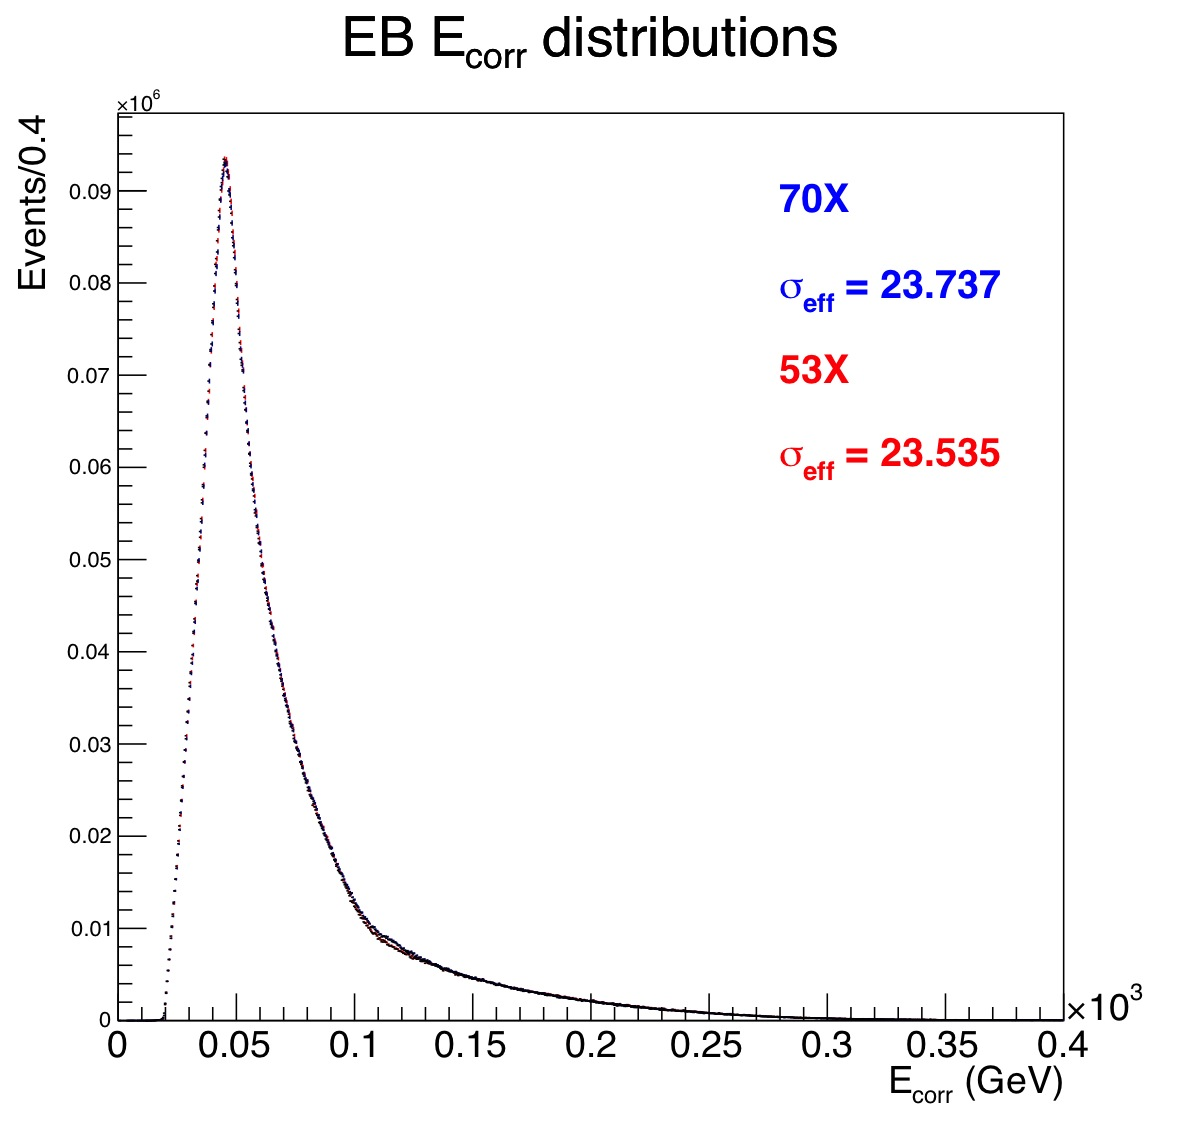
\includegraphics[width=\textwidth]{fullRunPlots/corrEnergySC_EB_dists}
                \caption{Distributions of $E_{\text{corr}}$ in the EB.}
                \label{distEB}
        \end{subfigure}
        \begin{subfigure}[b]{0.4\textwidth}
                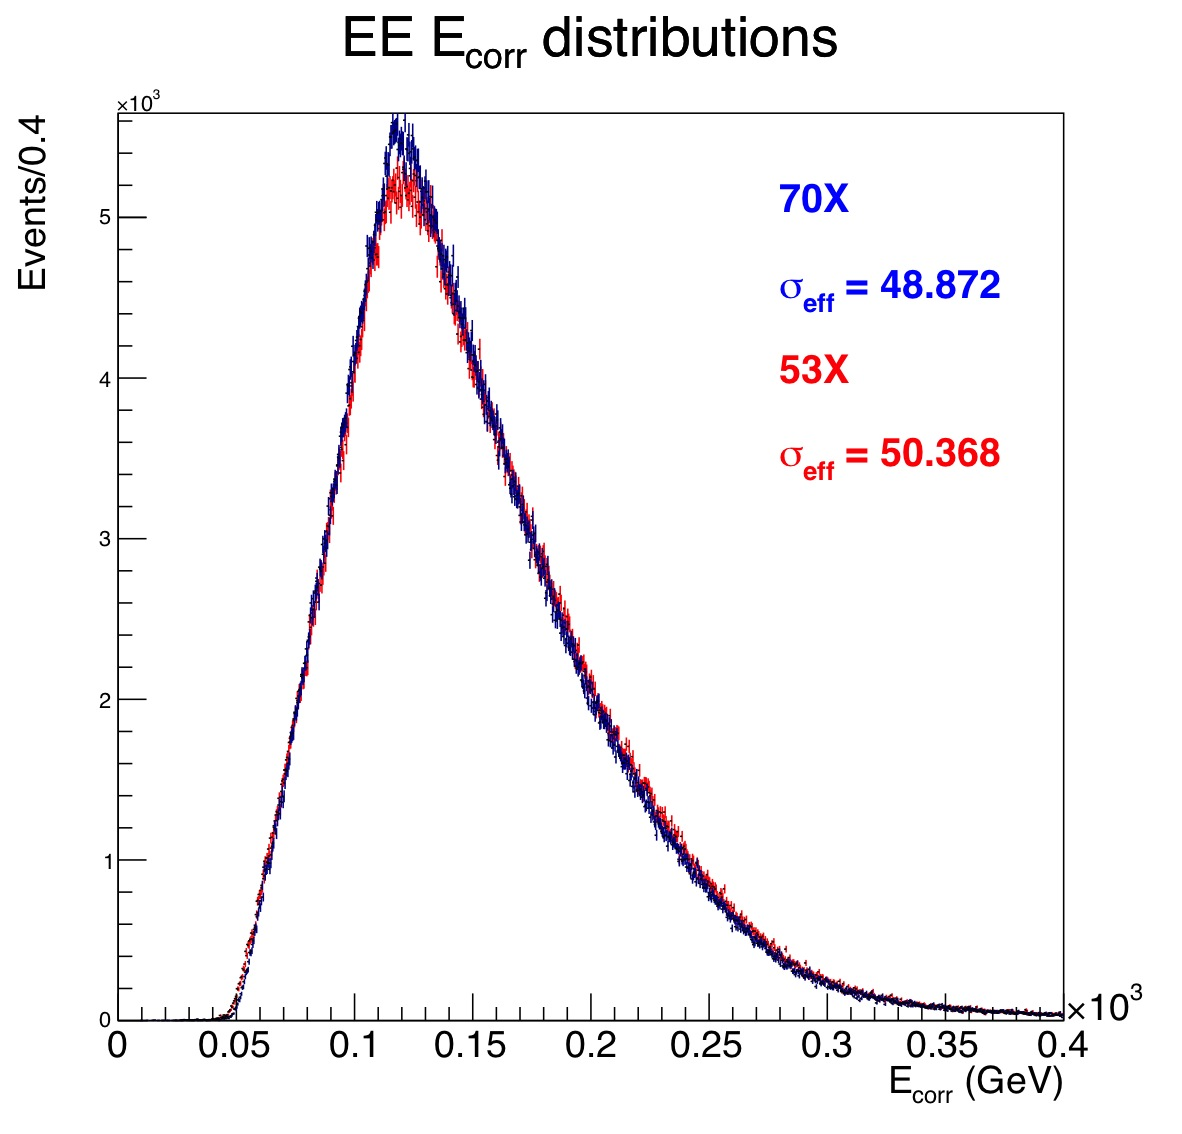
\includegraphics[width=\textwidth]{fullRunPlots/corrEnergySC_EE_dists}
                \caption{Distributions of $E_{\text{corr}}$ in the EE.}
                \label{distEE}
        \end{subfigure}
        \begin{subfigure}[b]{0.4\textwidth}
                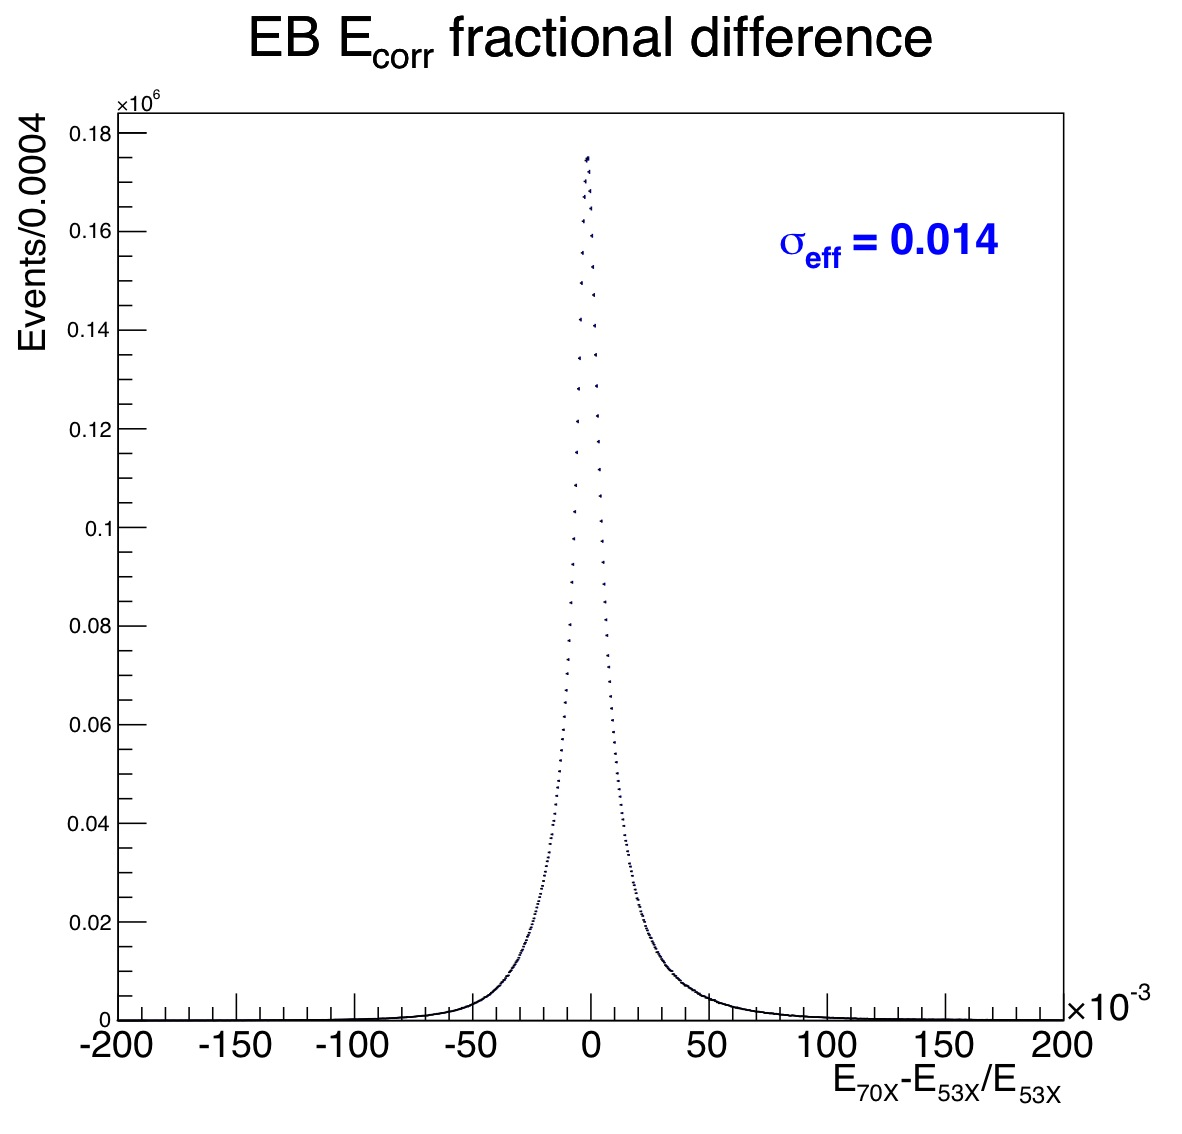
\includegraphics[width=\textwidth]{fullRunPlots/corrEnergySC_EB}
                \caption{Fractional change of $E_{\text{corr}}$ in the EB.}
                \label{chEB}            
        \end{subfigure}
         \begin{subfigure}[b]{0.4\textwidth}
                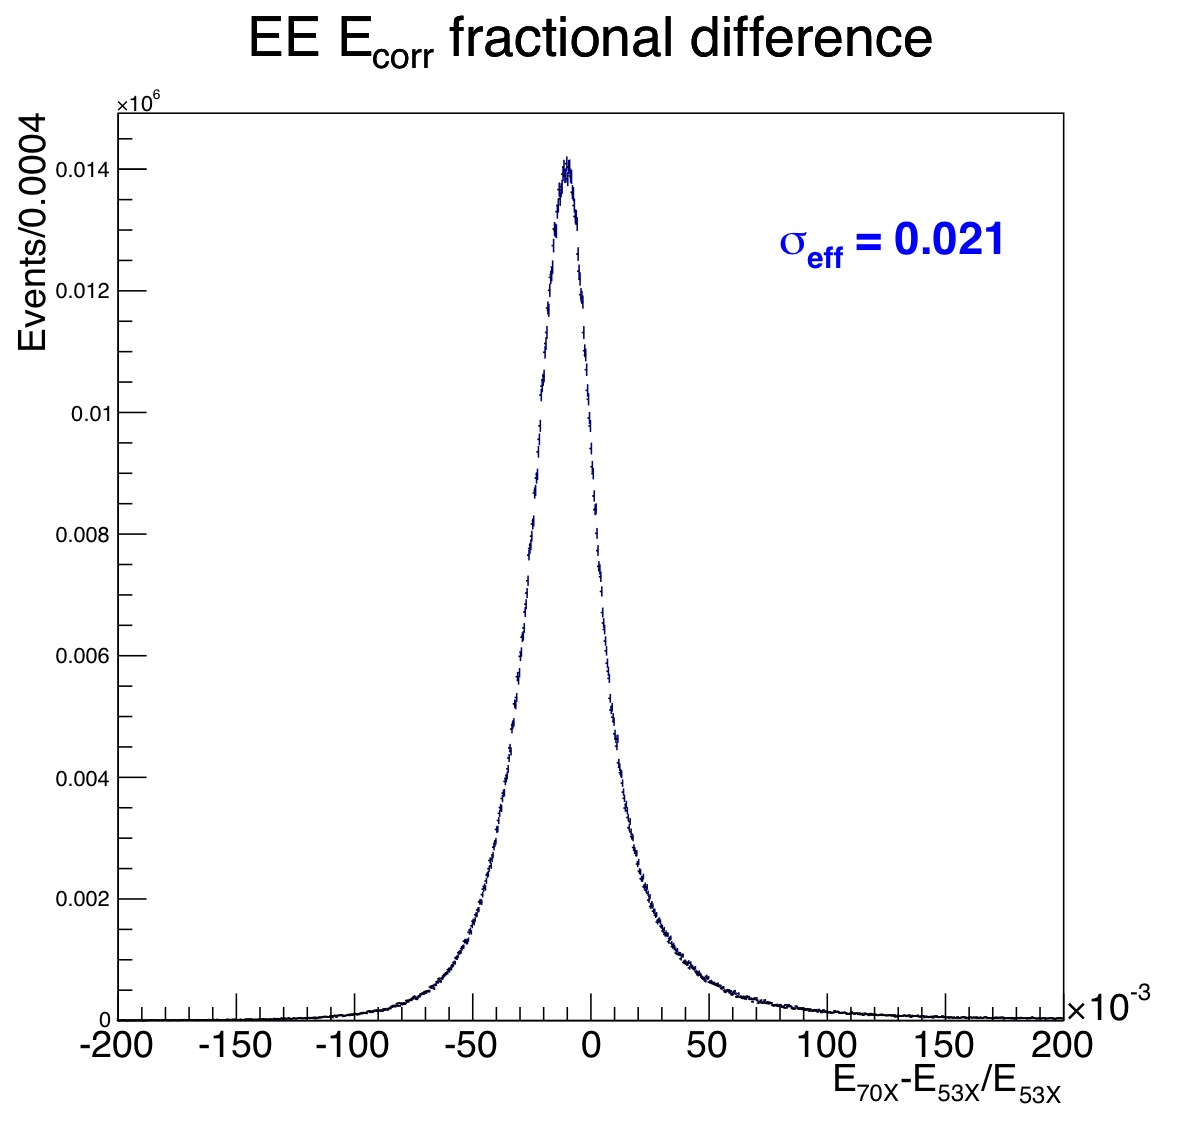
\includegraphics[width=\textwidth]{fullRunPlots/corrEnergySC_EE}
                \caption{Fractional change of $E_{\text{corr}}$ in the EE.}
                \label{chEE}
        \end{subfigure}
        \caption{ (\ref{distEB}) shows the distributions of corrected energy for the two frameworks in the barrel. (\ref{distEE}) shows the equivalent plot for the endcaps. (\ref{chEB}) shows the fractional energy difference $\frac{E_\texttt{70X} -E_\texttt{53X}}{E_\texttt{53X}}$ for electrons in the EB. (\ref{chEE}) shows the equivalent plot for the EE.}
        \label{energyValidation}
\end{figure}

The reconstruction of the energy of ECAL objects is clearly of paramount interest in this study. Fig. \ref{energyValidation} shows plots relating to the corrected energy, $E_{\text{corr}}$, in \texttt{53X} compared to \texttt{70X}. The corrected energy was chosen as the fairest way to compare the frameworks. However, it is worth noting that the corrected energy for \texttt{53X} is the ``best'' option available, while the corrected energy for \texttt{70X} is simply an initial attempt at correction, which is likely to improve greatly once the the sample is calibrated using the MC. Figs. \ref{distEB} and \ref{distEE} show the energy distributions for \texttt{70X} and \texttt{53X}. In the EB, the distributions from the two frameworks appear to agree well, apart from a feature around $\sim 120$ GeV which needs to be investigated further. For the EE, the distributions show inconsistencies, particularly at the peak, also at $\sim 120$ GeV. Figs. \ref{chEB} and \ref{chEE} show the fractional energy difference $(E_\texttt{70X}-E_\texttt{53X})/E_\texttt{53X}$ in the EB and EE. The figures indicate that the two frameworks do indeed tend to agree more closely in the EB compared to the EE.

\begin{figure}[h!]
        \centering
                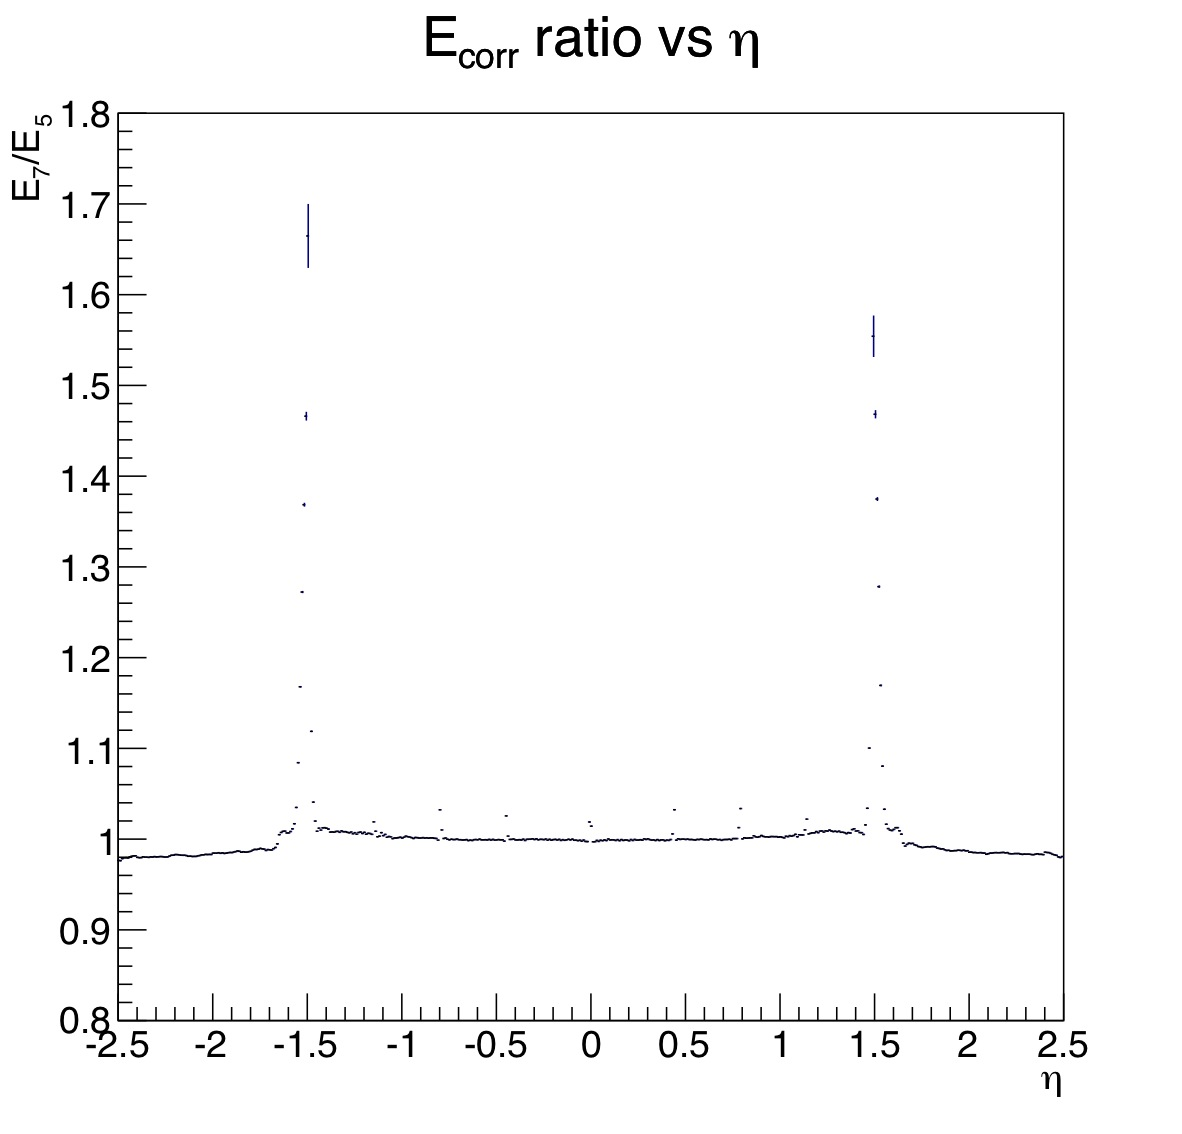
\includegraphics[width=0.5\textwidth]{fullRunPlots/corrE_profile}
                \caption{Ratio of corrected energies versus $\eta$.}
                \label{E_profile}
\end{figure}

The agreement in the barrel and disagreement in the endcaps can be seen very clearly in Fig. \ref{E_profile}, which shows the average value of $\frac{E_{\text{corr}\texttt{70X}}}{E_{\text{corr}\texttt{53X}}}$ as a function of $\eta$. In the region $|\eta|<1.5$, which represents the EB, the ratio is consistent with 1. However, for $|\eta|>1.5$ (in the EE), the ratio is consistently below 1, indicating that \texttt{70X} is underestimating the energy. A check was run to be certain that \texttt{53X} was not overestimating the energy: invariant mass distributions of $Z\rightarrow e^+ e^-$ electrons with at least one electron in the EE were plotted for both frameworks. The gaussian peak for $\texttt{53X}$ was near the nominal $Z$ mass as expected, while the peak  for $\texttt{70X}$ was indeed shifted down by $\sim 0.5$ GeV. The discrepancy in the EE needs to be further investigated with a deeper validation. Another interesting feature in Fig. \ref{E_profile} is that large discrepancies are observed at the interfaces between EE and EB (at $\eta = \pm 1.5$) and the module boundaries in the EB (at $|\eta| = 0.435, 0.783 \text{ and } 1.131$).% These discrepancies are explained by the fact that the regression in \texttt{70X} accounts for the losses at the module borders, while \texttt{53X} does not. 
\newpage
\subsubsection{$R_9$}
\begin{figure}[h!]
        \centering
        \begin{subfigure}[b]{0.37\textwidth}
                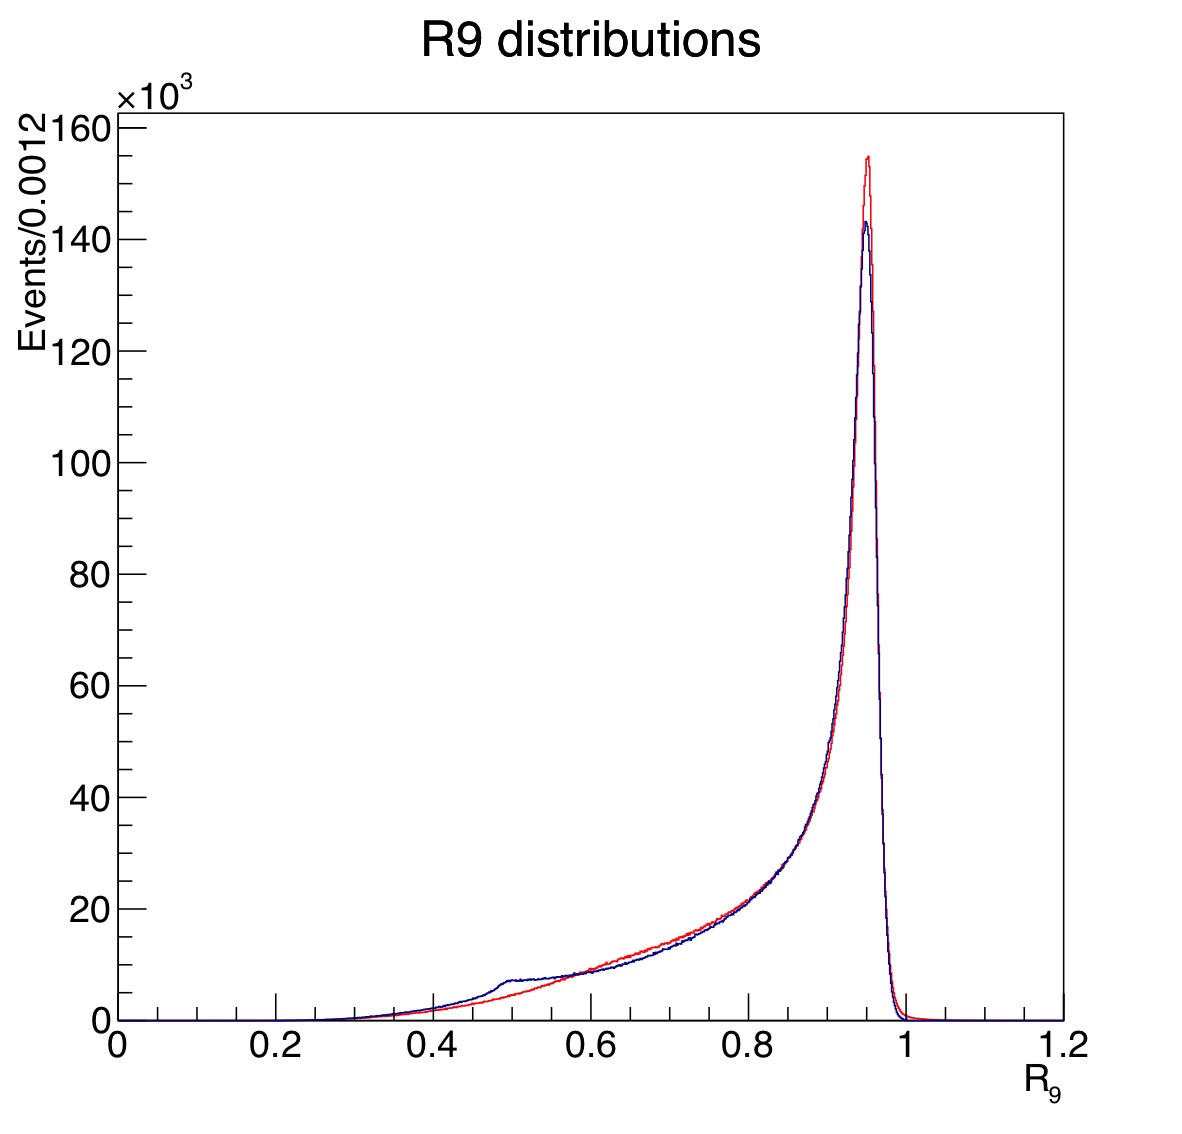
\includegraphics[width=\textwidth]{fullRunPlots/R9_dist}
                \caption{$R_9$ distributions: \texttt{53X} (red) \& \texttt{70X} (blue).}
                \label{r9Dist}
        \end{subfigure}%
        \quad\quad\quad
        \begin{subfigure}[b]{0.37\textwidth}
                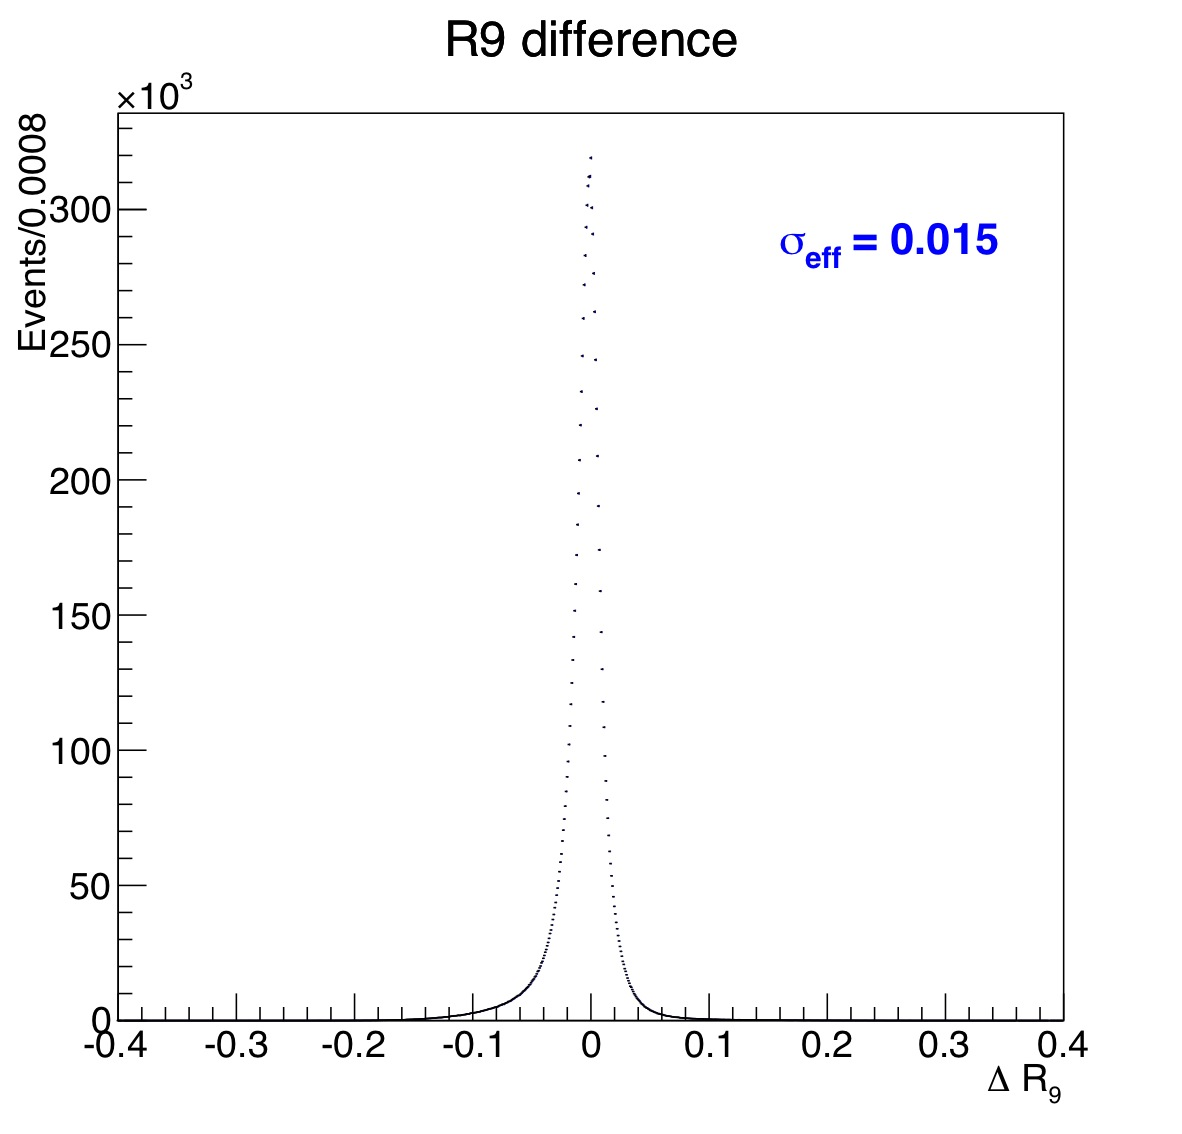
\includegraphics[width=\textwidth]{fullRunPlots/R9}
                \caption{The distribution of the difference in $R_9$.}
                \label{r9Diff}
        \end{subfigure}
       
        \caption{$R_9$ validation plots.}\label{r9Validation}
\end{figure}

For electrons, the interpretation of $R_9$ is different to that for photons. In this case, it indicates whether an electron is likely to have emitted a large fraction of its energy through bremsstrahlung or not. Electrons with $R_9>0.94$ are likely to have lost little energy. On the other hand, electrons with $R_9\leq 0.94$ will have little more of their energy before hitting the detector, and this might not be included in the supercluster. In this case, they are more difficult to reconstruct. Fig. \ref{r9Dist} shows the distribution of the $R_9$ values of electrons in the data samples. The red line refers to electrons reconstructed in \texttt{53X}, while the blue line shows the distributions of electrons reconstructed in \texttt{70X}. Only electrons which had a match from one sample to the other were included. The distributions match up well, apart from the peak, where the \texttt{70X} distribution is not as high, and around 0.5, where the \texttt{70X} distribution shows a bump. These features needs to be investigated further. Fig. \ref{r9Diff} shows the distribution of the difference in $R_9$ (i.e. $(R_9)_{70X} -(R_9)_{53X}$). This forms a tight peak around 0, indicative that the two versions are generally assigning the same value of $R_9$ to the electrons.

\subsubsection{$\eta,\phi$ coordinates}
\begin{figure}[h!]
        \centering
        \begin{subfigure}[b]{0.24\textwidth}
                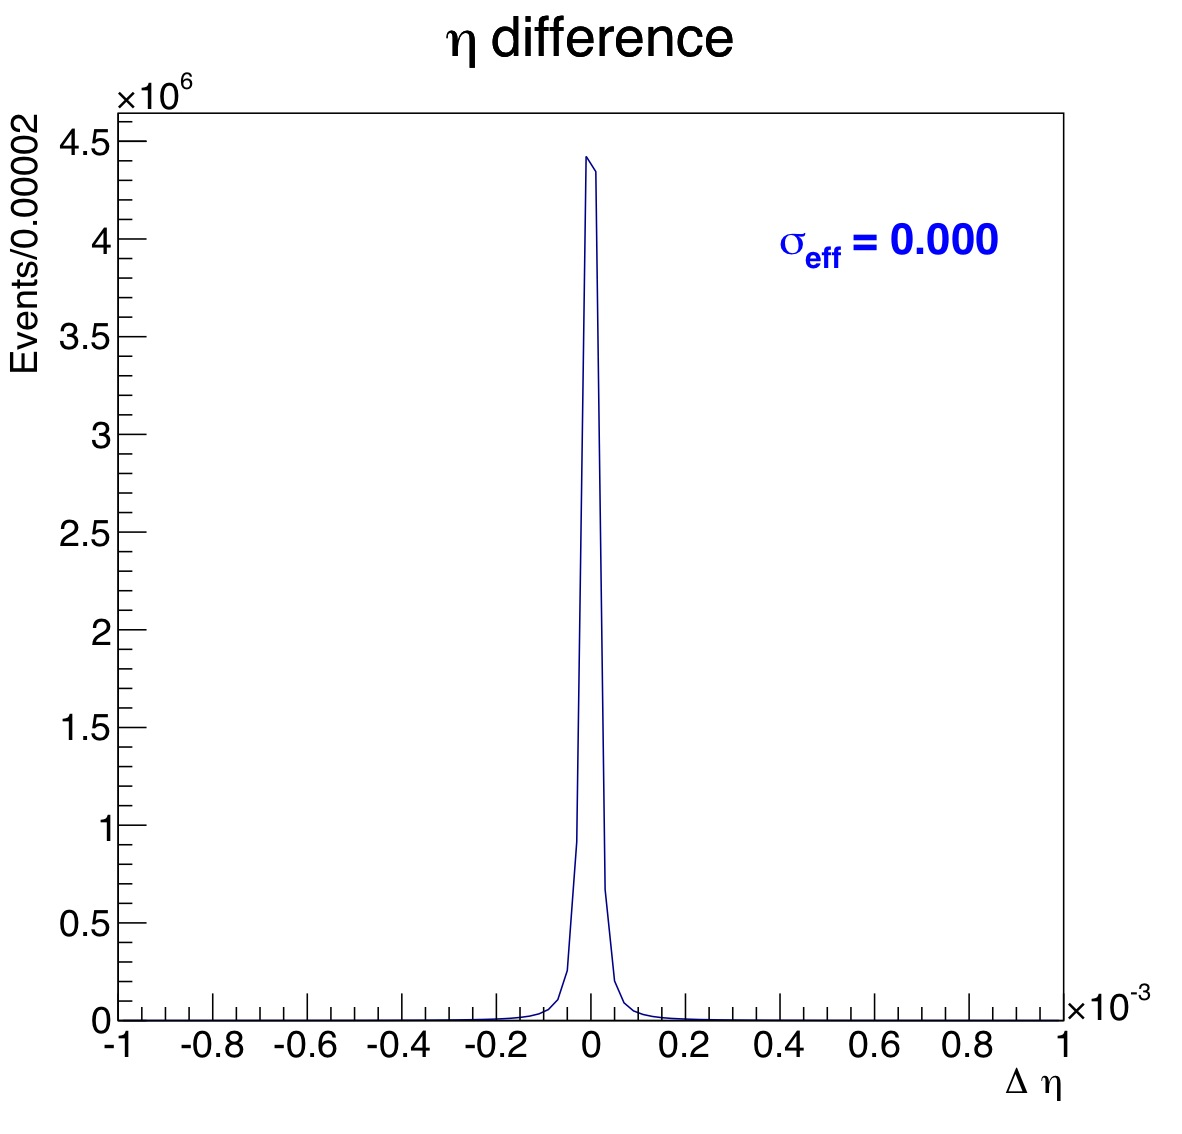
\includegraphics[width=\textwidth]{fullRunPlots/eta}
                \caption{$\eta$ of track direction.}
               
        \end{subfigure}%
        ~ %add desired spacing between images, e. g. ~, \quad, \qquad, \hfill etc.
          %(or a blank line to force the subfigure onto a new line)
        \begin{subfigure}[b]{0.24\textwidth}
                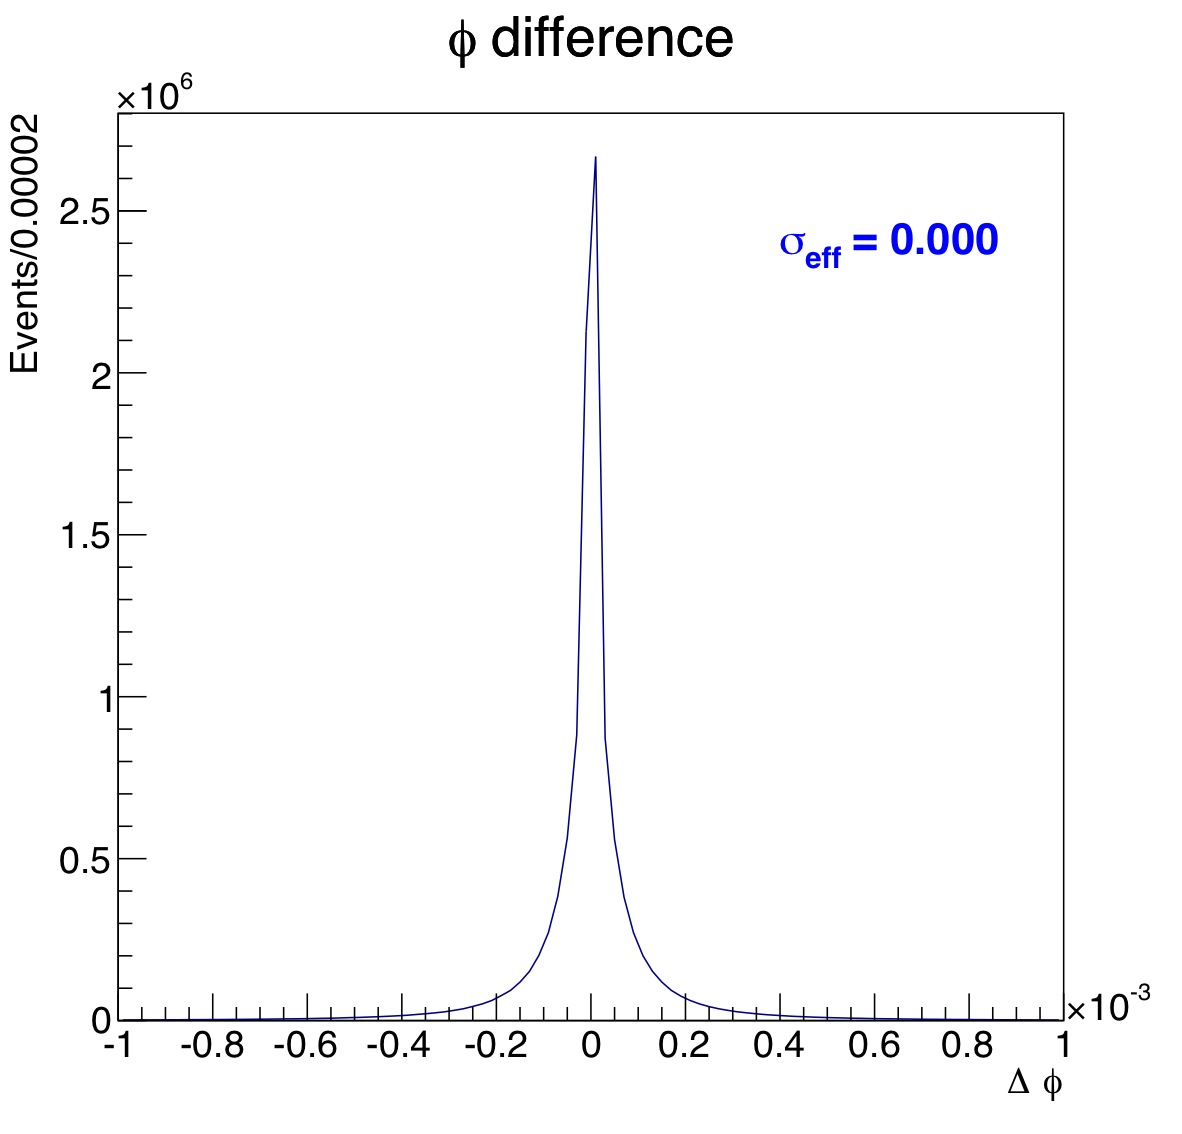
\includegraphics[width=\textwidth]{fullRunPlots/phi}
                \caption{$\phi$ of track direction.}
            
        \end{subfigure}
        ~ %add desired spacing between images, e. g. ~, \quad, \qquad, \hfill etc.
          %(or a blank line to force the subfigure onto a new line)
        \begin{subfigure}[b]{0.24\textwidth}
                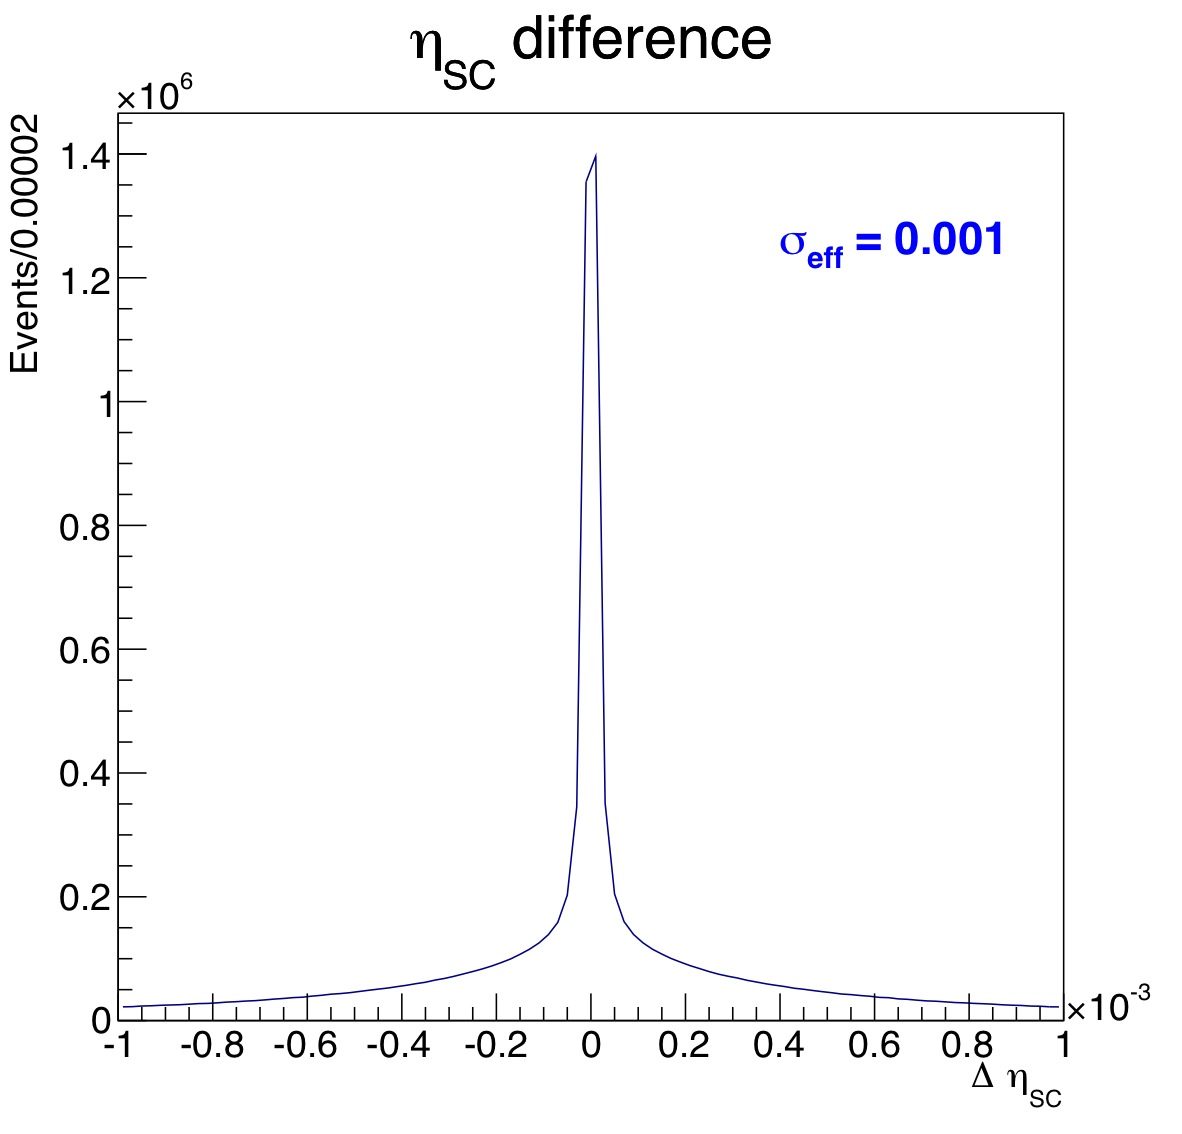
\includegraphics[width=\textwidth]{fullRunPlots/etaSC}
                \caption{$\eta$ of SC.}
            
        \end{subfigure}
         \begin{subfigure}[b]{0.24\textwidth}
                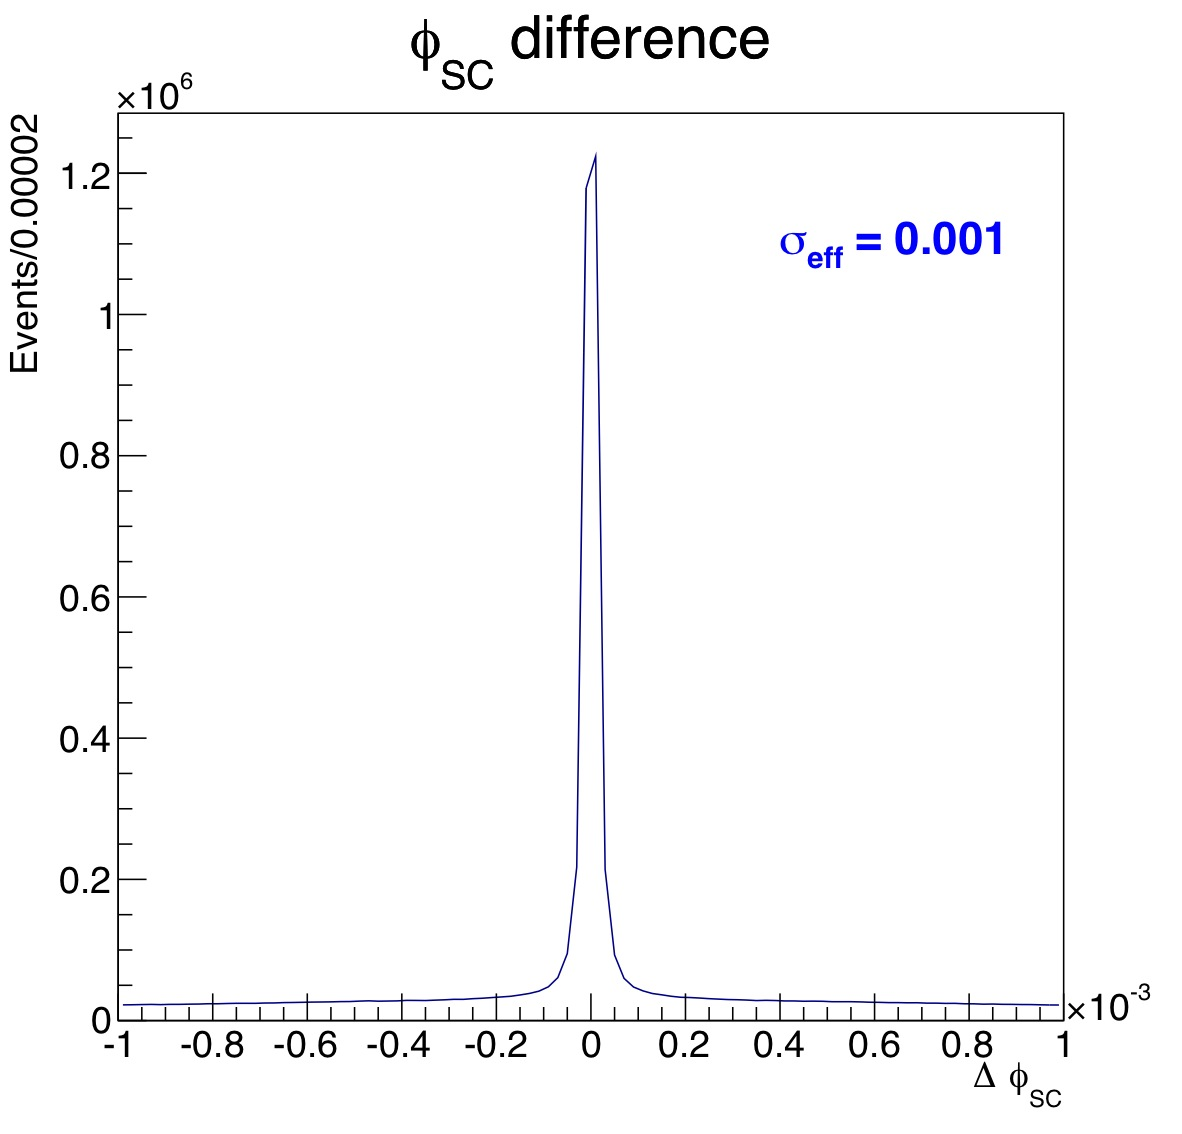
\includegraphics[width=\textwidth]{fullRunPlots/phiSC}
                \caption{$\phi$ of SC.}
             
        \end{subfigure}
        \caption{The distributions of $\Delta\eta,\Delta\phi$ for tracks and $\Delta\eta_{SC},\Delta\phi_{SC}$ for superclusters.}
        \label{posValidation}
\end{figure}

The position where the electrons hit the ECAL (known as the supercluster position $\eta_{\text{SC}},\phi_{\text{SC}}$) should not be largely affected by the change in framework, and neither should the coordinates of the electron tracks, in this case, known as $\eta,\phi$. The difference between the two is that $\eta_{\text{SC}},\phi_{\text{SC}}$ are measured from the centre of the detector, while $\eta,\phi$ start at the interaction vertex, and thus are shifted in the $z$-direction. Fig. \ref{posValidation} shows the distributions of the change in the value of $\eta_{\text{SC}},\phi_{\text{SC}},\eta \text{ and } \phi$. As expected, the distributions form extremely narrow peaks around zero. This indicates that indeed, the values of the coordinates remain largely unaffected. The values of $\eta_{\text{SC}},\phi_{\text{SC}}$ are more affected than $\eta,\phi$, but this makes sense, since $\eta_{\text{SC}},\phi_{\text{SC}}$ are the energy-weighted average of the coordinates of the crystals in the supercluster, and thus would be more affected by a change in clustering algorithm.


\subsubsection{$Z\rightarrow e^+ e^-$ invariant mass }
\begin{figure}[h]
        \centering
        \begin{subfigure}[b]{0.35\textwidth}
                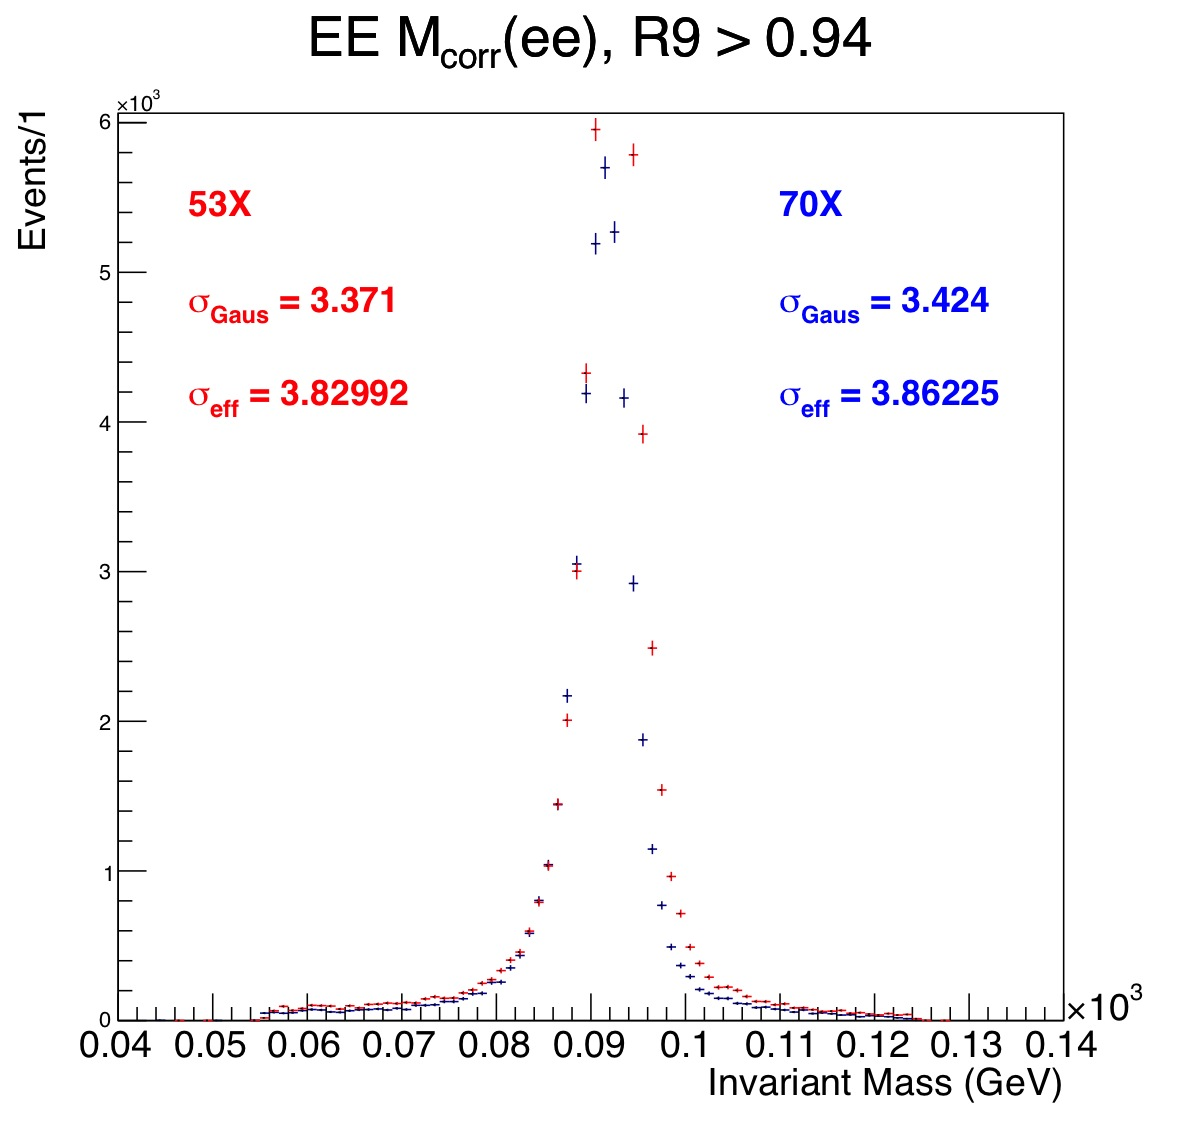
\includegraphics[width=\textwidth]{fullRunPlots/Zee_corr_1}
                \caption{}
        \end{subfigure}
         \begin{subfigure}[b]{0.35\textwidth}
                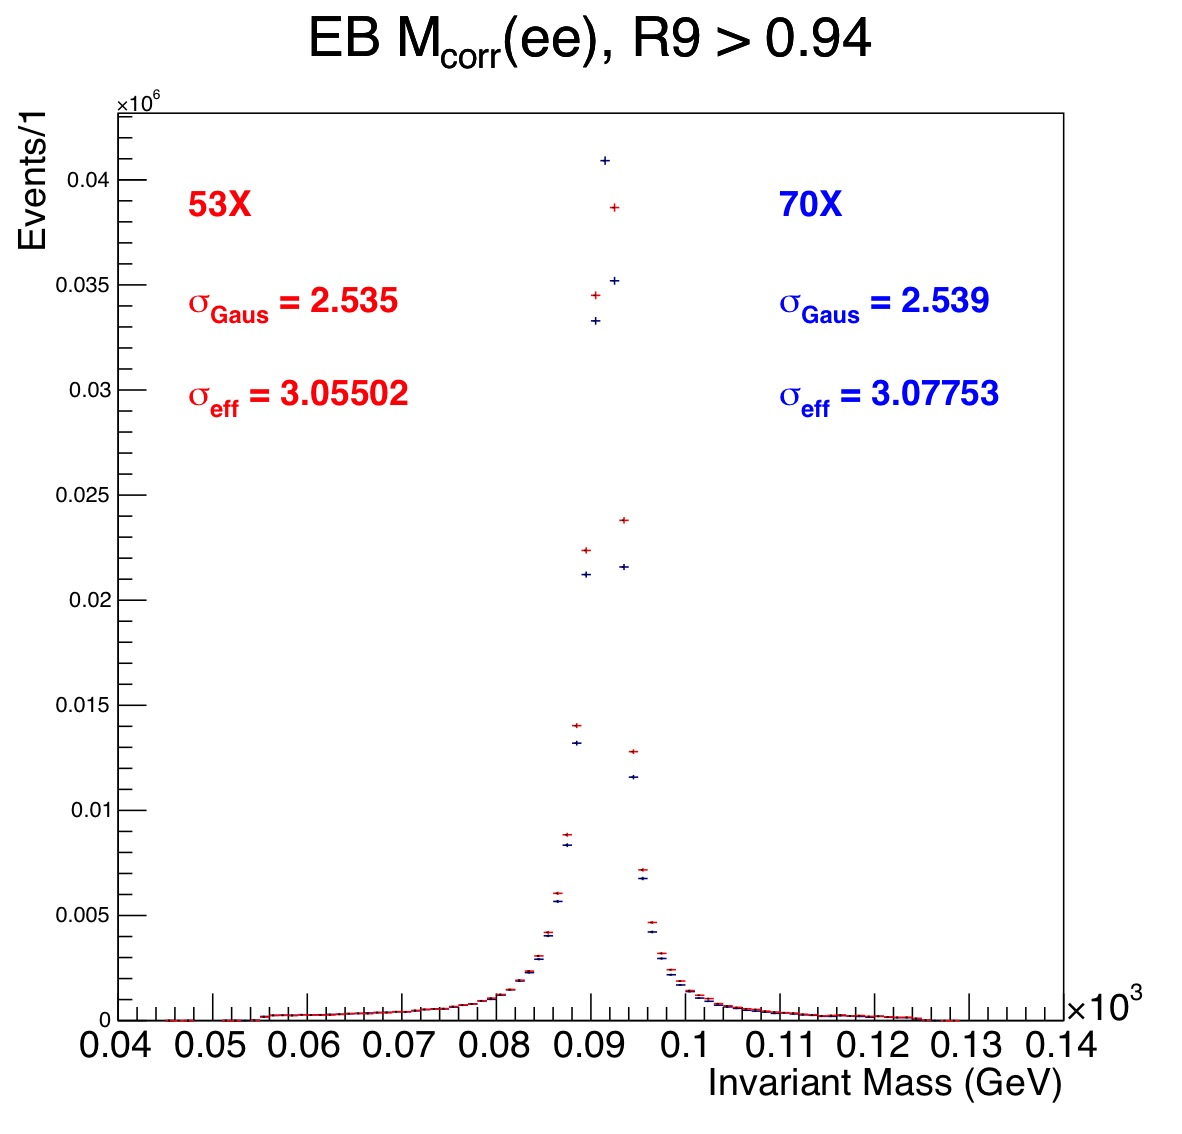
\includegraphics[width=\textwidth]{fullRunPlots/Zee_corr_2}
                  \caption{}
        \end{subfigure}
         \begin{subfigure}[b]{0.35\textwidth}
                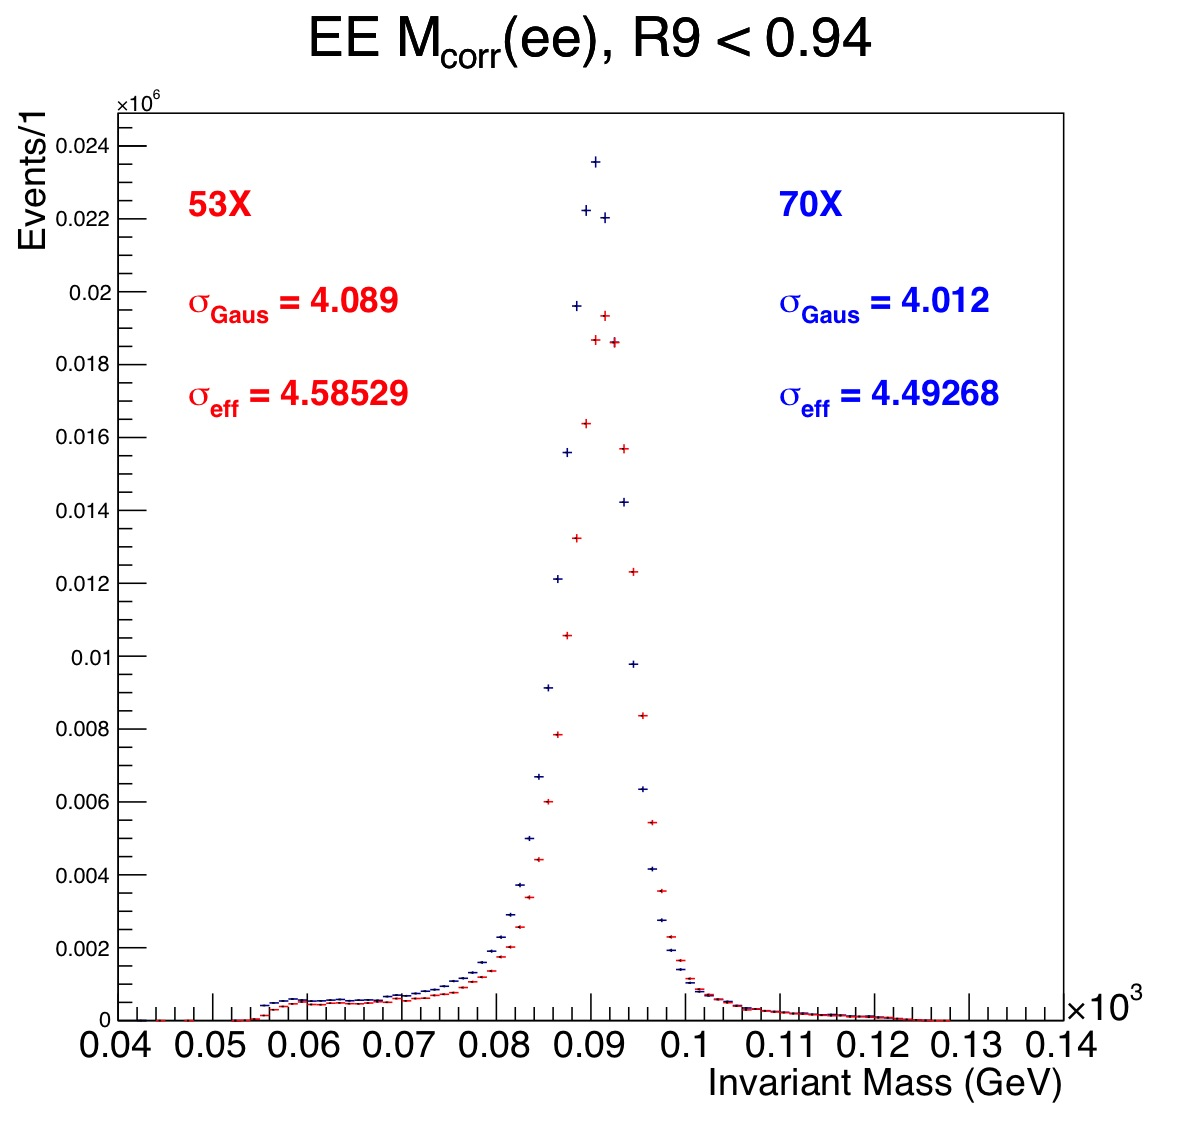
\includegraphics[width=\textwidth]{fullRunPlots/Zee_corr_3}
                  \caption{}
        \end{subfigure}
         \begin{subfigure}[b]{0.35\textwidth}
                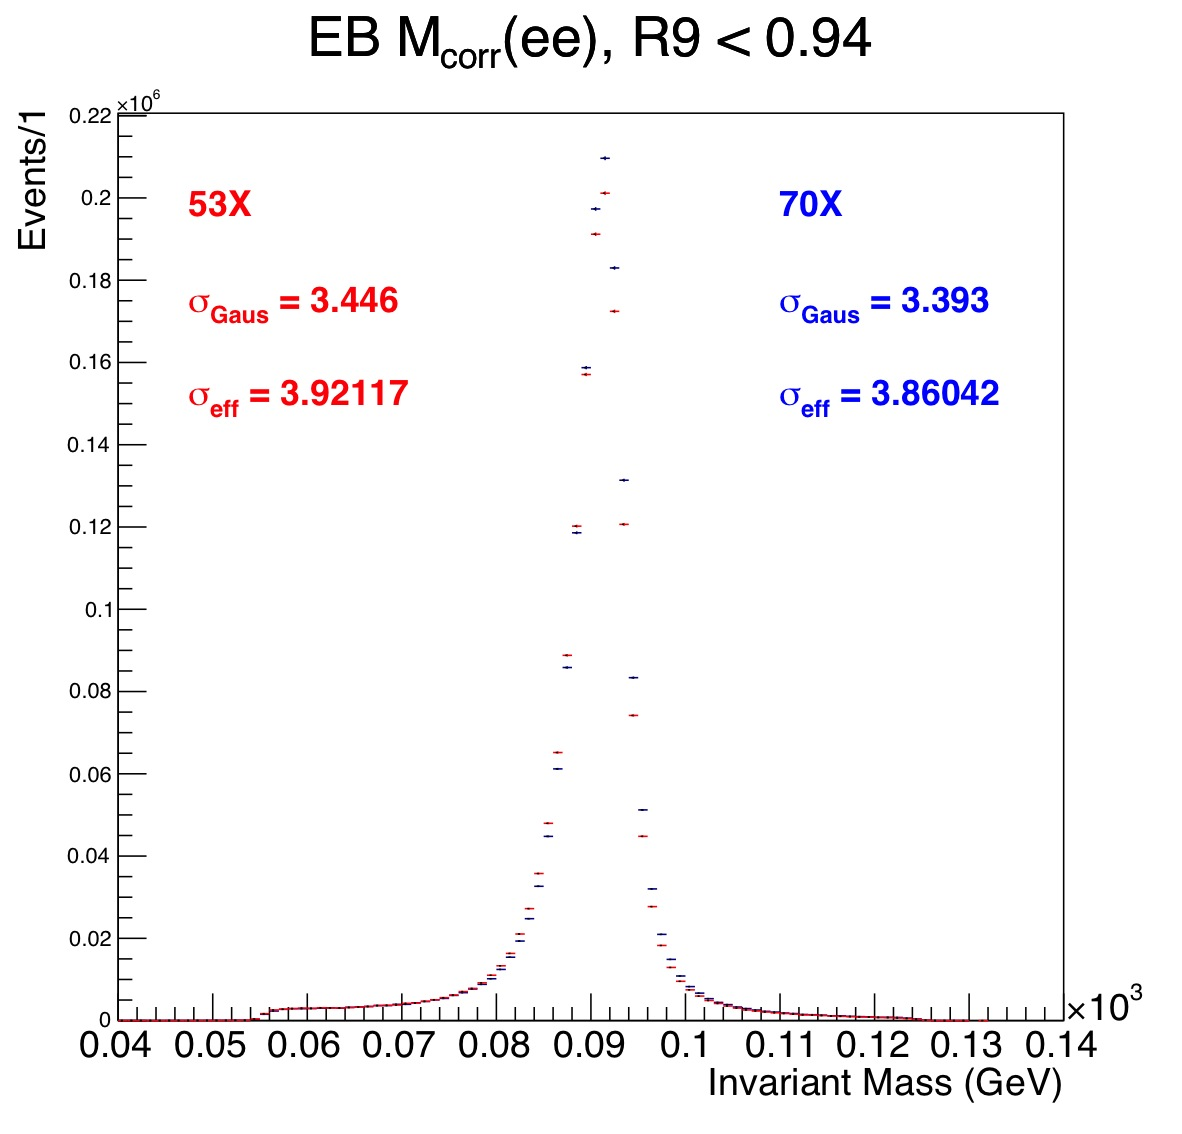
\includegraphics[width=\textwidth]{fullRunPlots/Zee_corr_4}
                  \caption{}
        \end{subfigure}
        \caption{Invariant mass distributions of $Z\rightarrow e^+e^-$ systems when both electrons are in the same $|\eta|,R_9$ category. The red histogram indicates \texttt{53X} while the blue histogram indicates \texttt{70X}.}\label{ZeeValidation}
\end{figure}

The invariant mass distributions of various categories of $Z \rightarrow e^+e^-$ system are shown in Fig. \ref{ZeeValidation}. There are four categories considered here: (a) both resulting electrons have $R_9 >0.94$ and are both in the EE, (b) both with $R_9>0.94$ and in the EB, (c) both with $R_9 \leq 0.94$ and in EE and (d) both with $R_9 \leq 0.94$ and in EB. The red lines indicate the distributions obtained when considering electrons in the \texttt{53X} frameworks, while the blue lines represent electrons from the \texttt{70X} version. Only matched electrons are included in this plot. The invariant mass is calculated using the corrected energy of the electrons - the best available for both \texttt{70X} and \texttt{53X}. The plots show good agreement in the two EB categories, where the two peaks overlap well, apart from the height of the peak. There is however a visible discrepancy in the EE, where the peaks appear shifted with respect to one another. Further investigation is needed to understand the differences observed.

%\subsection{Performance as a function of the number of primary vertices}

%\begin{figure}[h!]
%        \centering
 % 
   %             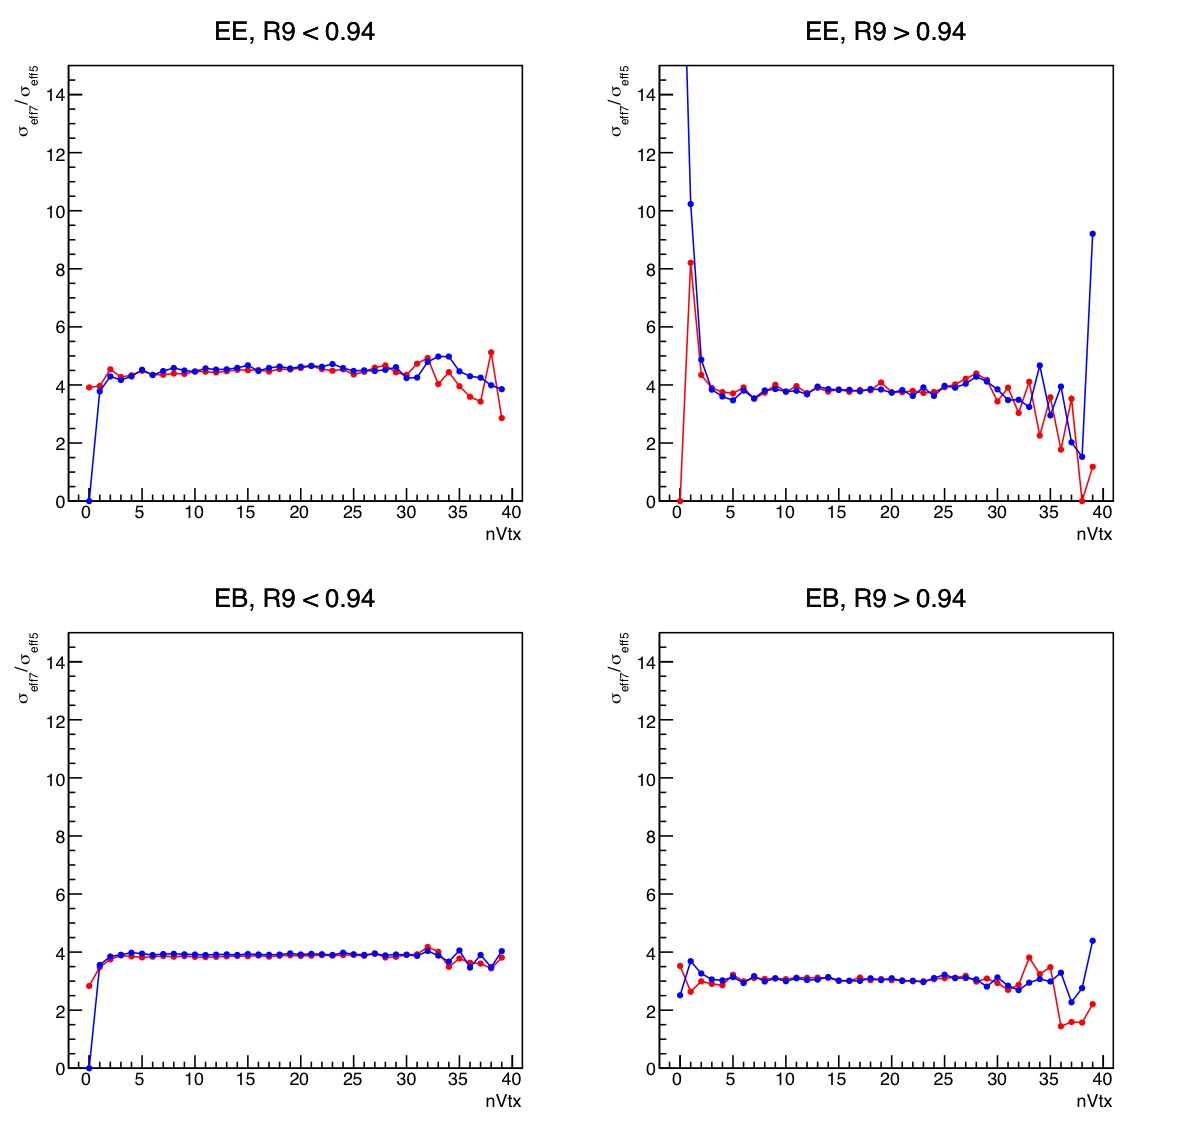
\includegraphics[width=0.7\textwidth]{fullRunPlots/effSigma_vs_nPV}
     %           \caption{}
  % 
    %    \caption{Ratio of $\sigma_{\text{eff}}$ in the $Z\rightarrow \e^+e^-$ as a function of the number of primary vertices in the event, for various locations and $R_9$ values. The}
     %   \label{npv}
%\end{figure}
%
%Finally, the ratios of the $\sigma_{\text{eff}}$ values of the $Z\rightarrow \e^+e^-$ distributions


\subsection{Next Steps}

This section has shown results from the preliminary steps of validation of the regression in the \texttt{70X} framework. At the moment, the comparisons are being made using data reconstructed in both \texttt{53X} and \texttt{70X}, but for full validation, matching MC samples are needed also. Although some variables appear to match (namely the $\eta_{\text{SC}},\phi_{\text{SC}},\eta \text{ and }\phi$), more studies are needed to probe differences observed between energy-based variables, particularly in the EE. The MC for the \texttt{70X} sample is due to become available shortly, so we will be able to run the \texttt{ECALELF} tool in its entirety, and thus provide a better correction for the \texttt{70X} energy. This new correction should allow a fairer comparison to be made. I am working with the ECAL DPG to pursue this work.


\section{Summary and conclusion}
The LHC should begin collisions again in 2015, and new data will then become available. Various new measurements will need to be made to further understand the properties of the Higgs boson. Further data will be able to shed light on the existence of a potential second Higgs boson (multiple such bosons are predicted in various BSM frameworks), and will allow precision measurements of differential cross sections, couplings and spin/parity. Deviations from the expected properties of the SM Higgs boson could signal the potential existence of BSM physics.  $H\rightarrow \gamma \gamma$ will remain one of the most sensitive channels with which to analyse the properties of the Higgs during run II. My work within the CMS experiment so far has been centred around the ECAL, preparing for run II. The way that photons and electrons are reconstructed is being modified, and I am helping to determine what the effect of this change will be on the sensitivity, particularly that of the $H \rightarrow \gamma \gamma$ analysis. As 2015 approaches, I will become involved in planning and implementing the next round of the  $H \rightarrow \gamma \gamma$ analysis, to help further pin down the properties of the Higgs boson.

To conclude, it is clear that even though we have now discovered the elusive Higgs boson, many questions remain unanswered. In 2015, some BSM theories which might help to answer these questions will be tested. If nothing is found in direct searches, the precision analysis of the properties of the Higgs boson will be one of key avenues with which to search for deviations from the SM. As such, further understanding of the Higgs boson's properties are not only desirable, but indeed imperative if we are to understand more about the fundamental structure of the universe. The key to performing these measurements is the good performance of the sub-detectors and preparation of the collaboration.


\bibliographystyle{unsrt}
\bibliography{mybib}
%\end{multicols}
\end{document}